\documentclass[14pt,a4paper]{report}  %紙張設定
\usepackage{xeCJK}%中文字體模組
%\setCJKmainfont{標楷體} %設定中文字體
\setCJKmainfont{MoeStandardKai.ttf}
%\newfontfamily\sectionef{Times New Roman}%設定英文字體
\newfontfamily\sectionef{Nimbus Roman}
\usepackage{enumerate}
\usepackage{amsmath,amssymb}%數學公式、符號
\usepackage{amsfonts} %數學簍空的英文字
\usepackage{graphicx, subfigure}%圖形
\usepackage{fontawesome5} %引用icon
\usepackage{type1cm} %調整字體絕對大小
\usepackage{textpos} %設定文字絕對位置
\usepackage[top=2.5truecm,bottom=2.5truecm,
left=3truecm,right=2.5truecm]{geometry}
\usepackage{titlesec} %目錄標題設定模組
\usepackage{titletoc} %目錄內容設定模組
\usepackage{textcomp} %表格設定模組
\usepackage{multirow} %合併行
%\usepackage{multicol} %合併欄
\usepackage{CJK} %中文模組
\usepackage{CJKnumb} %中文數字模組
\usepackage{wallpaper} %浮水印
\usepackage{listings} %引用程式碼
\usepackage{hyperref} %引用url連結
\usepackage{setspace}
\usepackage{lscape}%設定橫式
\lstset{language=Python, %設定語言
		basicstyle=\fontsize{10pt}{2pt}\selectfont, %設定程式內文字體大小
		frame=lines,	%設定程式框架為線
}
%\usepackage{subcaption}%副圖標
\graphicspath{{./../images/}} %圖片預設讀取路徑
\usepackage{indentfirst} %設定開頭縮排模組
\renewcommand{\figurename}{\Large 圖.} %更改圖片標題名稱
\renewcommand{\tablename}{\Large 表.}
\renewcommand{\lstlistingname}{\Large 程式.} %設定程式標示名稱
\hoffset=-5mm %調整左右邊界
\voffset=-8mm %調整上下邊界
\setlength{\parindent}{3em}%設定首行行距縮排
\usepackage{appendix} %附錄
\usepackage{diagbox}%引用表格
\usepackage{multirow}%表格置中
%\usepackage{number line}
%=------------------更改標題內容----------------------=%
\titleformat{\chapter}[hang]{\center\sectionef\fontsize{20pt}{1pt}\bfseries}{\LARGE 第\CJKnumber{\thechapter}章}{1em}{}[]
\titleformat{\section}[hang]{\sectionef\fontsize{18pt}{2.5pt}\bfseries}{{\thesection}}{0.5em}{}[]
\titleformat{\subsection}[hang]{\sectionef\fontsize{18pt}{2.5pt}\bfseries}{{\thesubsection}}{1em}{}[]
%=------------------更改目錄內容-----------------------=%
\titlecontents{chapter}[11mm]{}{\sectionef\fontsize{18pt}{2.5pt}\bfseries\makebox[3.5em][l]
{第\CJKnumber{\thecontentslabel}章}}{}{\titlerule*[0.7pc]{.}\contentspage}
\titlecontents{section}[18mm]{}{\sectionef\LARGE\makebox[1.5em][l]
{\thecontentslabel}}{}{\titlerule*[0.7pc]{.}\contentspage}
\titlecontents{subsection}[4em]{}{\sectionef\Large\makebox[2.5em][l]{{\thecontentslabel}}}{}{\titlerule*[0.7pc]{.}\contentspage}
%=----------------------章節間距----------------------=%
\titlespacing*{\chapter} {0pt}{0pt}{18pt}
\titlespacing*{\section} {0pt}{12pt}{6pt}
\titlespacing*{\subsection} {0pt}{6pt}{6pt}
%=----------------------標題-------------------------=%             
\begin{document} %文件
\sectionef %設定英文字體啟用
\vspace{12em}
\begin{titlepage}%開頭
\begin{center}   %標題  
\makebox[1.5\width][s] %[s] 代表 Stretch the interword space in text across the entire width
{\fontsize{24pt}{2.5pt}國立虎尾科技大學}\\[18pt]
\makebox[1.5\width][s]
{\fontsize{24pt}{2.5pt}機械設計工程系}\\[18pt]
\sectionef\fontsize{24pt}{1em}\selectfont\textbf
{
\vspace{0.5em}
cd2023 2a3-pj3ag5分組報告}\\[18pt]
%設定文字盒子 [方框寬度的1.5倍寬][對其方式為文字平均分分布於方框中]\\距離下方18pt
\vspace{1em} %下移
\fontsize{30pt}{1pt}\selectfont\textbf{網際手足球場景設計}\\
\vspace{1em}
\sectionef\fontsize{30pt}{1em}\selectfont\textbf
{
\vspace{0.5em}
Web-based Foosball Scene Design}
 \vspace{2em}
%=---------------------參與人員-----------------------=%             
\end{center}
\begin{flushleft}
\begin{LARGE}

\hspace{32mm}\makebox[5cm][s]
{指導教授:\quad 嚴\quad 家\quad 銘\quad 老\quad 師}\\[6pt]
\hspace{32mm}\makebox[5cm][s]
{班\qquad 級:\quad 四\quad 設\quad 二\quad 甲}\\[6pt]
\hspace{32mm}\makebox[5cm][s]
{學\qquad 生:\quad 第\quad 一\quad 位\quad(41023154)組長}
\\[6pt]
\hspace{32mm}\makebox[5cm][s]
{\hspace{36.5mm}第\quad 二\quad 位\quad(41023135)}\\[6pt]
\hspace{32mm}\makebox[5cm][s]
{\hspace{36.5mm}第\quad 三 \quad 位\quad(41023140)}\\[6pt]
\hspace{32mm}\makebox[5cm][s]
{\hspace{36.5mm}第\quad 四 \quad 位\quad(41023133)}\\[6pt]
\hspace{32mm}\makebox[5cm][s]
{\hspace{36.5mm}第\quad 五 \quad 位\quad(41023105)}\\[6pt]
\hspace{32mm}\makebox[5cm][s]
{\hspace{36.5mm}第\quad 六 \quad 位\quad(41023107)}\\[6pt]
\hspace{32mm}\makebox[5cm][s]
{\hspace{36.5mm}第\quad 七 \quad 位\quad(41023102)}\\[6pt]
\hspace{32mm}\makebox[5cm][s]
{\hspace{36.5mm}第\quad 八 \quad 位\quad(41023109)}\\[6pt]
%設定文字盒子[寬度為5cm][對其方式為文字平均分分布於方框中]空白距離{36.5mm}\空白1em
\end{LARGE}
\end{flushleft}
\vspace{6em}
\fontsize{18pt}{2pt}\selectfont\centerline{\makebox[\width][s]
{中華民國\hspace{3em} 
112 \quad 年\quad 6\quad 月}}
\end{titlepage}
\newpage
%=---------------報告製作核可證明---------------------=%
 {\renewcommand\baselinestretch{1.4}\selectfont %設定以下行距
 {\begin{center}
    {\fontsize{20pt}{2.5pt} {國立虎尾科技大學 \qquad 機械設計工程系}\\[8pt]{分組報告製作合格認可證明}\\
    \hspace*{\fill} \\ %似enter鍵換行
    \par}
     \end{center}}
    {\begin{textblock}{60}(1.85,0.8)
    \noindent \fontsize{15pt}{16pt}\selectfont 分組報告製作修習學生\enspace:\quad
    {\begin{minipage}[t]{10em}\underline{四設二甲\enspace 41023154 第一位}\\ \underline{四設二甲\enspace 41023135\enspace 第二位}\\ 
    \underline{四設二甲\enspace 41023140\enspace 第三位}\\
    \underline{四設二甲\enspace 41023133\enspace 第四位}\\
    \underline{四設二甲\enspace 41023105\enspace 第五位}\\
    \underline{四設二甲\enspace 41023107\enspace 第六位}\\
    \underline{四設二甲\enspace 41023102\enspace 第七位}\\
    \underline{四設二甲\enspace 41023109\enspace 第八位}\\
   %下劃線符號指令
    \end{minipage}}
         \par} %結束指定行距
    {\renewcommand\baselinestretch{1.2}\selectfont %設定以下行距
    {\begin{textblock}{30}(1.8,5)
    \noindent \fontsize{16pt}{16pt}\selectfont 分組報告題目\enspace :網際手足球場景設計
    \hspace*{\fill} \\
    \hspace*{\fill} \\
    \noindent \fontsize{16pt}{16pt}\selectfont 經評量合格,特此證明
    \hspace*{\fill} \\
    \hspace*{\fill} \\
    \noindent \fontsize{16pt}{16pt} \makebox[6em][s]{評審委員}\enspace:\quad
    {\begin{minipage}[t]{6em} \underline{            }\\[16pt] \underline{            }\\[16pt] \underline{            }\\
    \end{minipage}}
    \end{textblock}}
    {\begin{textblock}{10}(1.8,9)
    {\begin{flushleft}
    \fontsize{16pt}{16pt}\selectfont \makebox[6em][s]{指導老師}\enspace:\quad \underline{嚴家銘}\\[10pt]
    \hspace*{\fill} \\
    \fontsize{16pt}{2.5pt}\selectfont \makebox[12em][s]{中華民國一一二年}\hspace{2pt}
    \fontsize{16pt}{2.5pt}\selectfont\makebox[8em][s]{六月四日}
    \end{flushleft}}
    \end{textblock}}
    \end{textblock}}
     \par} %結束指定行距
     \newpage

%=------------------------摘要-----------------------=%
\renewcommand{\baselinestretch}{1.5} %設定行距
\pagenumbering{roman} %設定頁數為羅馬數字
\clearpage  %設定頁數開始編譯
\sectionef
\addcontentsline{toc}{chapter}{摘~~~要} %將摘要加入目錄
\begin{center}
\LARGE\textbf{摘~~要}\\
\end{center}
\begin{flushleft}
\fontsize{14pt}{20pt}\sectionef\hspace{12pt}\quad 本學期採取個人及團體分組來學習,學習團隊合作,團體協同開發一款能在
web-based CoppeliaSim 場景中雙方或多方對玩的遊戲。
\\[12pt]

\fontsize{14pt}{20pt}\sectionef\hspace{12pt}\quad 除了設計 bubbleRob 機器人、繪製球場、設定感測器及寫程式,我覺得最重要的是學會組員間的溝通及分配工作,大家各司其職才能共同做好這份作業。\\[12pt]

\end{flushleft}
\begin{flushleft}
\fontsize{14pt}{20pt}\selectfont 此專題是利用八台 BubbleRob 雙輪車分兩組在一足球場景中進行對戰,雙
方球門分別設有感測器,雙方共有八名 BubbleRob 進行比賽。在規定時間
內,每進一球即透過程式重新從球場中線發球,但球員位置不變,並重啟賽局。模擬場景中
還須配置實體計分板顯示比賽剩餘時間與比分。在 CoppeliaSim 模擬環境中
進行測試運用上的可行性並嘗試透過埠號供使用者觀看。
\end{flushleft}
\newpage
%=--------------------Abstract----------------------=%
\renewcommand{\baselinestretch}{1.5} %設定行距
\addcontentsline{toc}{chapter}{Abstract} %將摘要加入目錄
\begin{center}
\LARGE\textbf\sectionef{Abstract}\\
\begin{flushleft}
\fontsize{14pt}{16pt}\sectionef\hspace{12pt}\quad In this semester, individuals and groups are used to study, learn teamwork, and the group collaborates to develop a
Games played against two or more parties in a web-based CoppeliaSim scenario.\\[12pt]

\fontsize{14pt}{16pt}\sectionef\hspace{12pt}\quad In addition to designing the bubbleRob robot, drawing the field, setting sensors and writing programs, I think the most important thing is to learn how to communicate and assign work among team members.\\
\end{flushleft}
\begin{flushleft}
\fontsize{14pt}{16pt}\selectfont\sectionef This topic is to use eight BubbleRob two-wheeled vehicles to divide into two groups to compete in a football scene.
There are sensors on each of the square goals, and a total of eight BubbleRobs compete on both sides. at the specified time
Inside, every time a goal is scored, the ball will be served from the center line of the court through the program, but the players' positions will remain unchanged, and the game will be restarted. simulation scene
It is also necessary to configure the physical scoreboard to display the remaining time and score of the game. In the CoppeliaSim simulation environment
Test the feasibility of the application and try to make it available for users to watch through the port number.
\end{flushleft}
\newpage
%=------------------------目錄----------------------=%
\renewcommand{\contentsname}{\centerline{\fontsize{18pt}{\baselineskip}\selectfont\textbf{目\quad 錄}}}
\tableofcontents  %目錄產生
\newpage
%=------------------圖表目錄產生----------------------=%
\renewcommand{\listfigurename}{\centerline{\fontsize{18pt}{\baselineskip}\selectfont\textbf{圖\quad 目\quad 錄 }}}
\newcommand{\loflabel}{圖} %定義\loflabel 文字為圖
\renewcommand{\numberline}[1]{\loflabel~#1\hspace*{0.5em}}
\listoffigures
%\newcommand{\captioname}{圖}
\newpage
\renewcommand{\listtablename}{\centerline{\fontsize{18pt}{\baselineskip}\selectfont\textbf{表\quad 目\quad 錄 }}}
\newcommand{\lotlabel}{表} %定義\lotlabel 文字為表
\renewcommand{\numberline}[1]{\lotlabel~#1\hspace*{0.5em}}
\listoftables

\end{center}
%=-------------------------內容----------------------=%
\chapter{前言}
\renewcommand{\baselinestretch}{10.0} %設定行距
\pagenumbering{arabic} %設定頁號阿拉伯數字
\setcounter{page}{1}  %設定頁數
\fontsize{14pt}{2.5pt}\sectionef
\section{整體架構}
    經過討論後,我們將整個BubbleRob分為三大主題,分別為 「 SolidWorks 」 、「 CoppeliaSim 」 、「 Lua 」,再分數個小主題去完成本次競賽。下圖為本次競賽整體架構(圖.\ref{fig.機器人報告表格})\\

\begin{figure}[hbt!]
\begin{center}
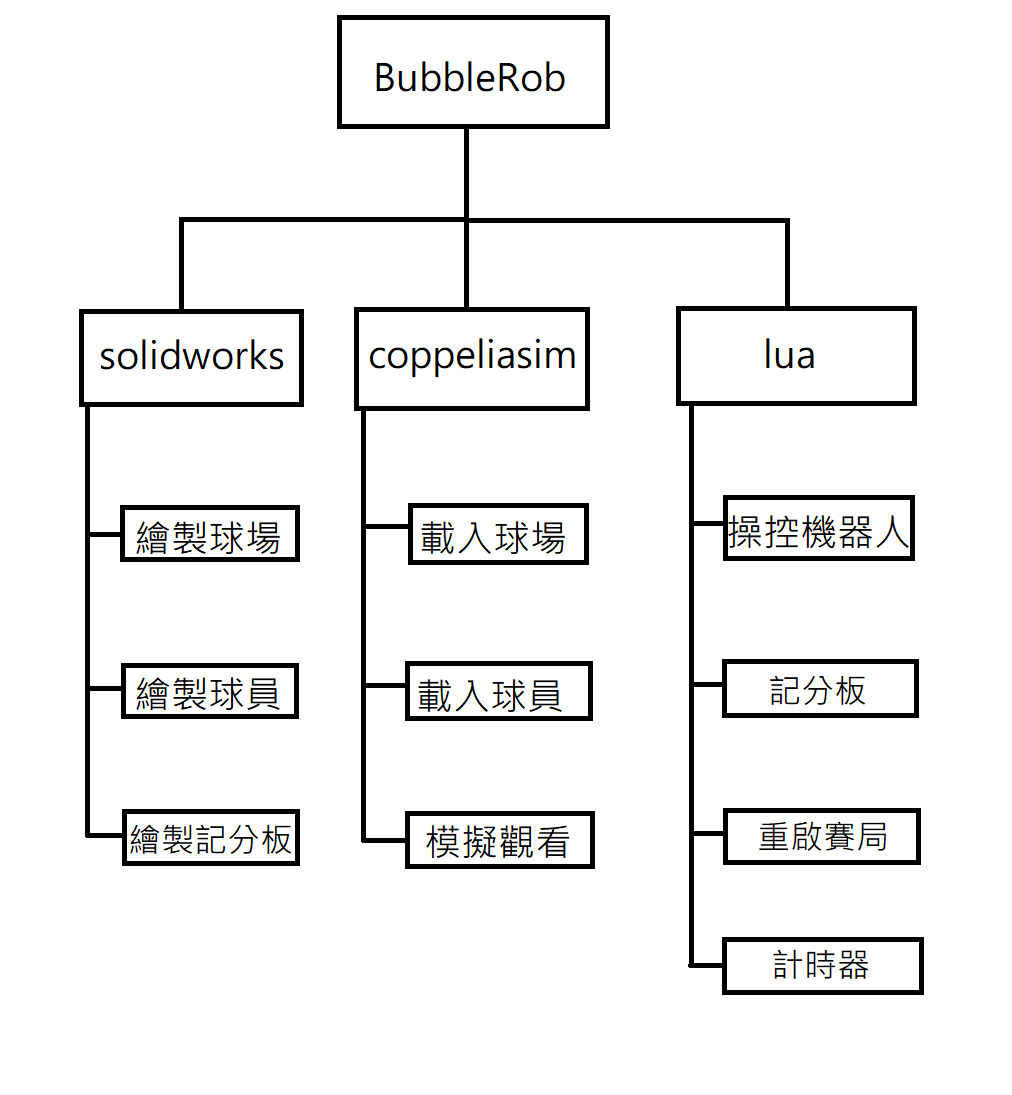
\includegraphics[width=13cm]{機器人報告表格}
\caption{\Large 心智圖}\label{fig.機器人報告表格}
\end{center}
\end{figure}


\section{研究目的與方法}
本研究分三大部分,第一運用OpenAI Gym裡內建編譯的ATARI 2600遊戲Pong-v0,來作為訓練環境,加上強化學習的理論,測試不同演算法參數以訓練出最佳化的對打系統,第二將整個簡化後冰球機導入CoppilaSim模擬環境並嘗試進行虛擬訓練,成為優化的對打機電系統。第三則是嘗試透過架設伺服器與虛擬環境結合。\\
 
透過簡化實體冰球機並導入虛擬環境,進行虛擬訓練,使用Gym的Pong當作對應的2D虛擬訓練環境,測試算法和訓練效果,篩選適合的算法與參數。\\

建置CoppilaSim模擬環境,嘗試將2D訓練概念套用到3D環境進行測試,加入電腦視覺與RemoteAPI,電腦視覺抓取球與擊錘的位置,透過RemoteAPI進行遠端控制,在3D環境測試算法可確保後續套用到實體機器上的可行性。\\
 
 再透過架設伺服器與虛擬環境結合:讓虛擬環境的影像透過網伺服器串流影像供使用者遠端進行操控虛擬環境的擊錘進行打球,或是提供多人進行觀看對打影像。
\begin{figure}[hbt!]
\begin{center}
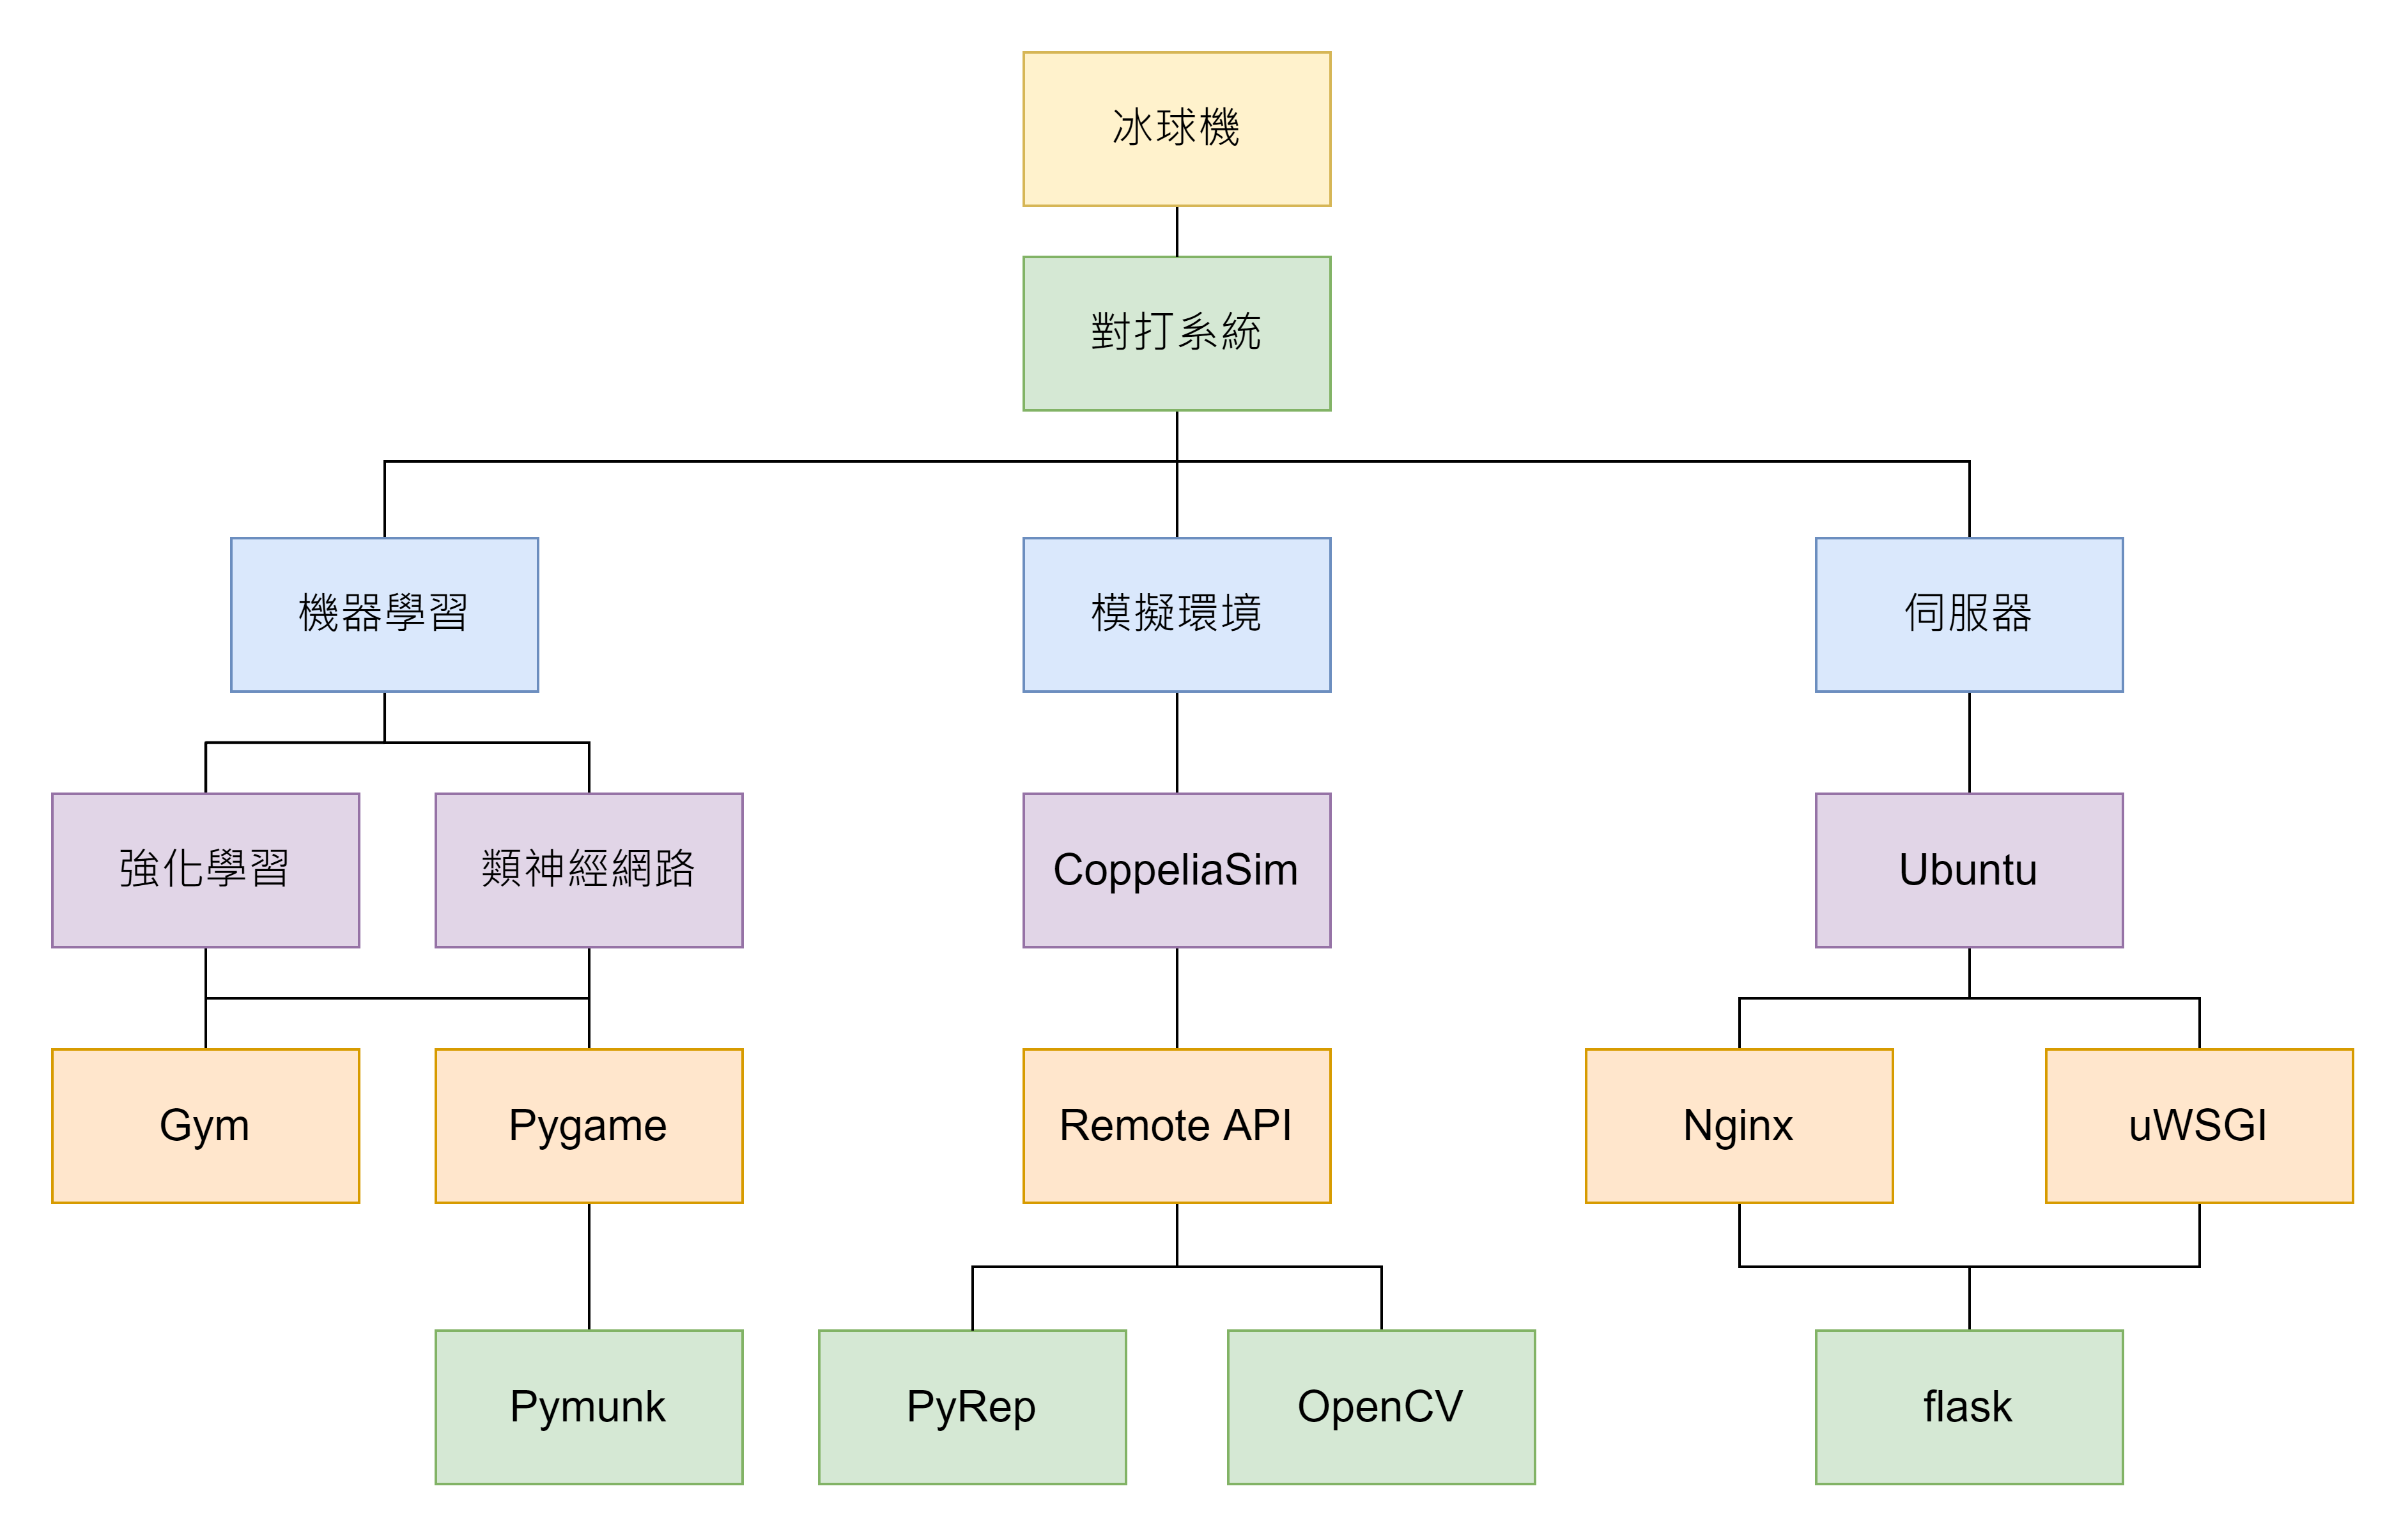
\includegraphics[width=15cm]{研究架構}
\caption{\Large 研究架構 }
\label{研究架構 }
\end{center}
\end{figure}
\section{未來展望}
此專題希望能利用現有完成的機械學習的算法,能發展成虛擬訓練,再將訓練完的機器學習應用到虛擬環境或是實體機電系統,並透過伺服器將影像串流提供玩家網頁介面進行遠端操控,同時提供多人觀看及時的比賽影像,將整個冰球機的控制和使用者間有更完善串聯,機電系統的部分達到最優化控制和虛實整合的應用。
\section{規則說明}
 Pong game 的遊戲規則簡單,透過擊錘將球打入對方球門即得一分,只要其中一方得21分就結束該局。擊錘只能沿單方向來回移動來進行防守和進攻。\\
遊戲規則如下:
\begin{enumerate}
\item 球打入敵方即得一分。
\item 擊錘只單一方向移動。
\item 最快贏得21分者獲勝,並結束該局遊戲。
\end{enumerate}

\renewcommand{\baselinestretch}{0.5} %設定行距
\chapter{球員設計}
\section{設計概念}
    原先球員設計是一人設計一種球員,但經過討論後,發現如果一人一種機器人會造成整個場面很混亂,所以最後選擇分成兩對,一隊一種球員設計。使用上述方法,觀看者可以更好的分辨隊伍,操作者也能明確地確認隊友。\\[6pt]

\section{球員設計(一)}
    球員一採用縮小本體體積,兩側伸出較長的竿子阻饒敵人搶球,且能更好的控制球。如(圖.\ref{球員})\\[6pt]\\
\begin{figure}[hbt!]
\center
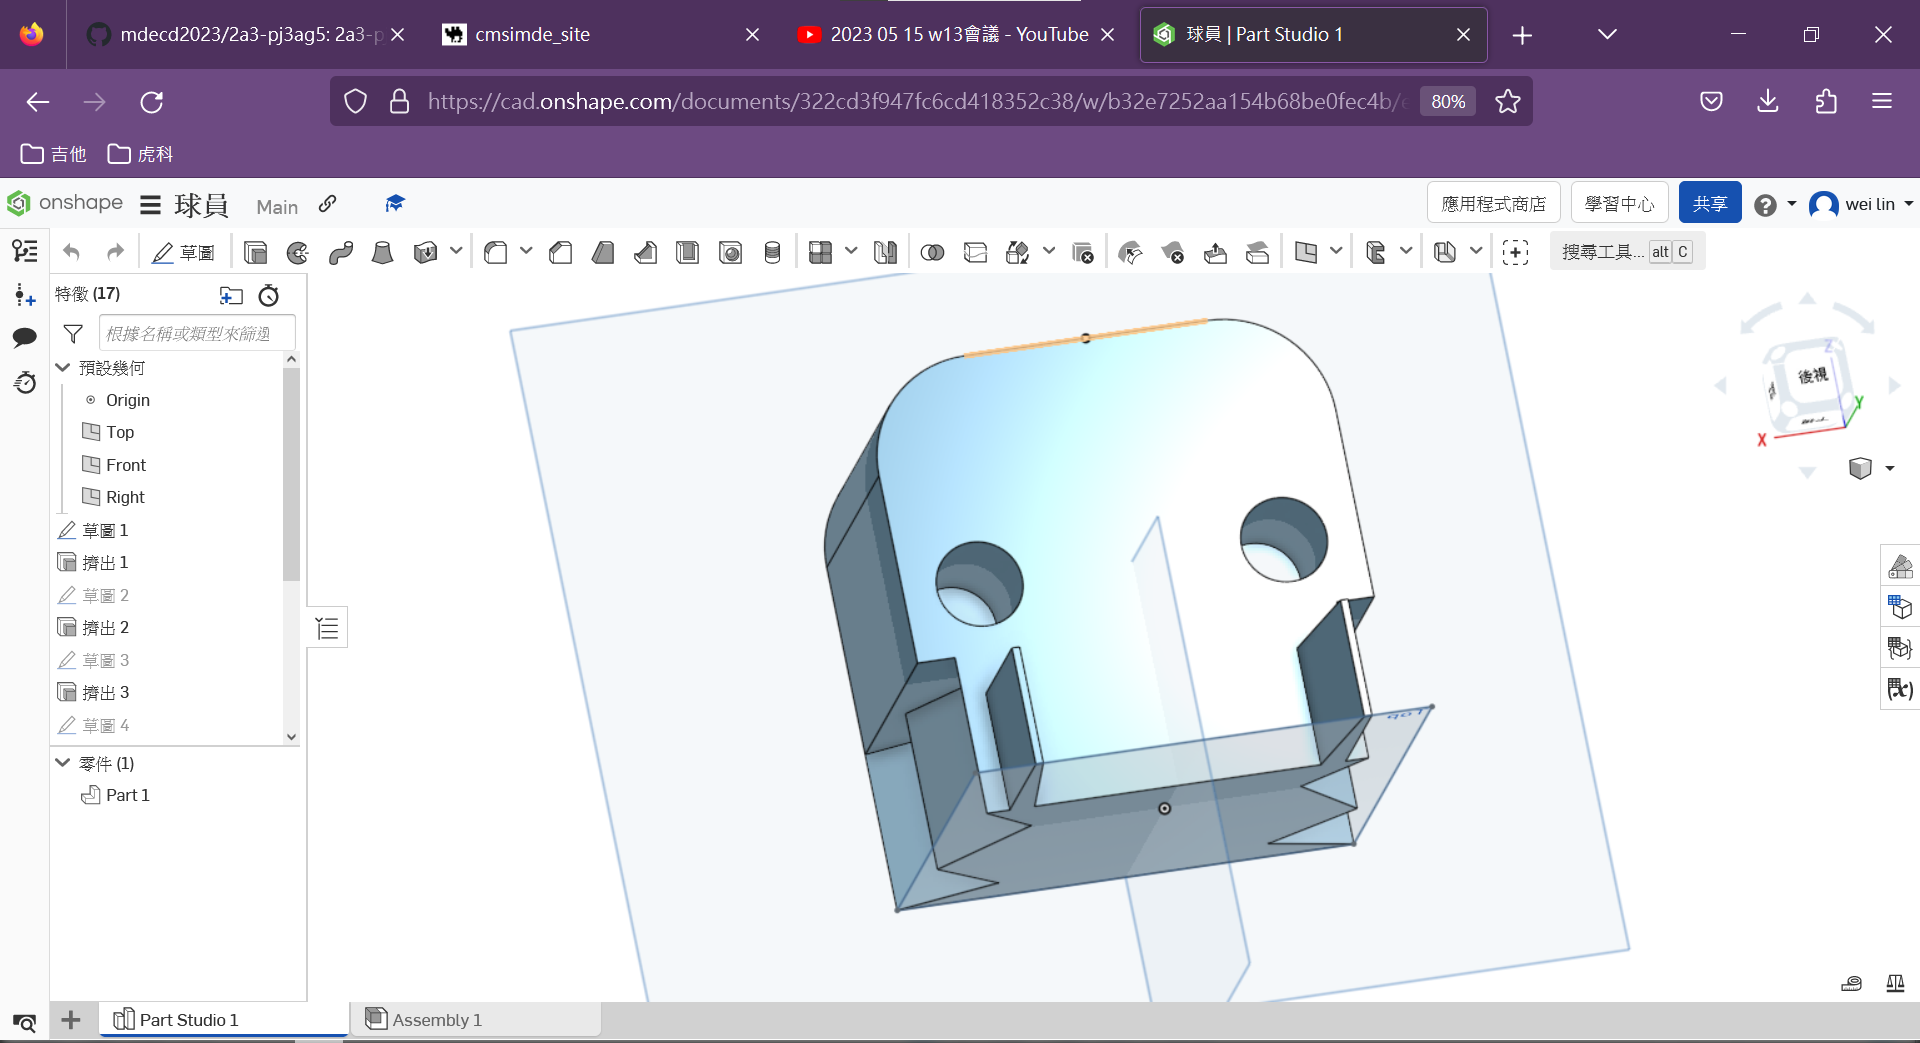
\includegraphics[width=13cm]{球員}
\caption{\Large 球員(一)}
\label{球員}
\end{figure}
\chapter{場景設計}
\section{設計理念}
 當初會想到這樣畫是因為想要更接近實際的樣貌,所以才會多做一個觀眾席和路燈。想讓這個遊戲玩起來更真實,更貼近生活。\\[6pt]
\begin{figure}[hbt!]
\begin{center}
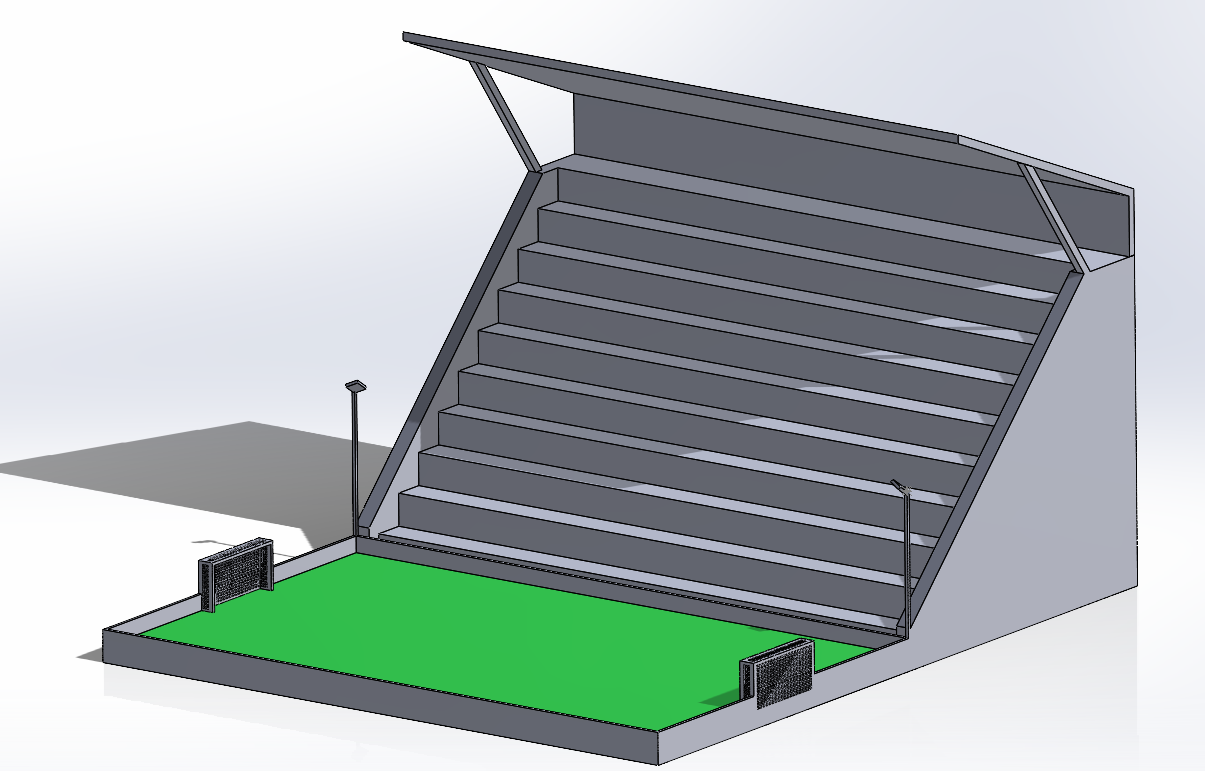
\includegraphics[height=6cm]{場景}
\caption{\Large 場景}\label{場景}
\end{center}
\end{figure} 

\section{設計更改}

將原本的場景放入CopppeliaSim時,因為球門的網格太細而出現模型計算的問題,導致在執行程式或操控球員時,會發生很嚴重的延遲。修改過後將球門設為平滑面,再執行一次就沒有模型計算問題了。\\[6pt]

\begin{figure}[hbt!]
\begin{center}
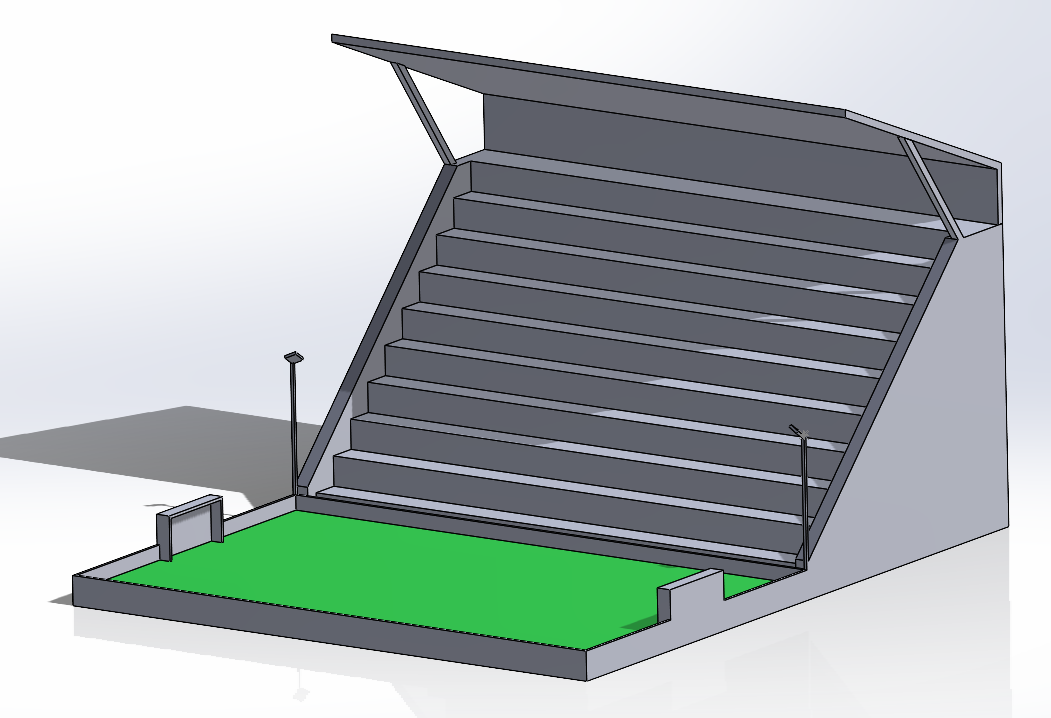
\includegraphics[height=6cm]{場景new}
\caption{\Large 修改後場景}\label{場景new}
\end{center}
\end{figure} 

\newpage
\chapter{記分板設計}
%\renewcommand{\baselinestretch}{10.0} %設定行距
\section{設計概念}
    依老師要求採用機械轉盤傳動計分系統,由齒輪帶動個位數及十位數的數字轉盤,再搭配程式驅動,使其能夠輕鬆且準確的計算分數,圖為我們自己製作的計分板。(圖.\ref{機械轉盤傳動計分系統})\\
    
\begin{figure}[hbt!]
\center
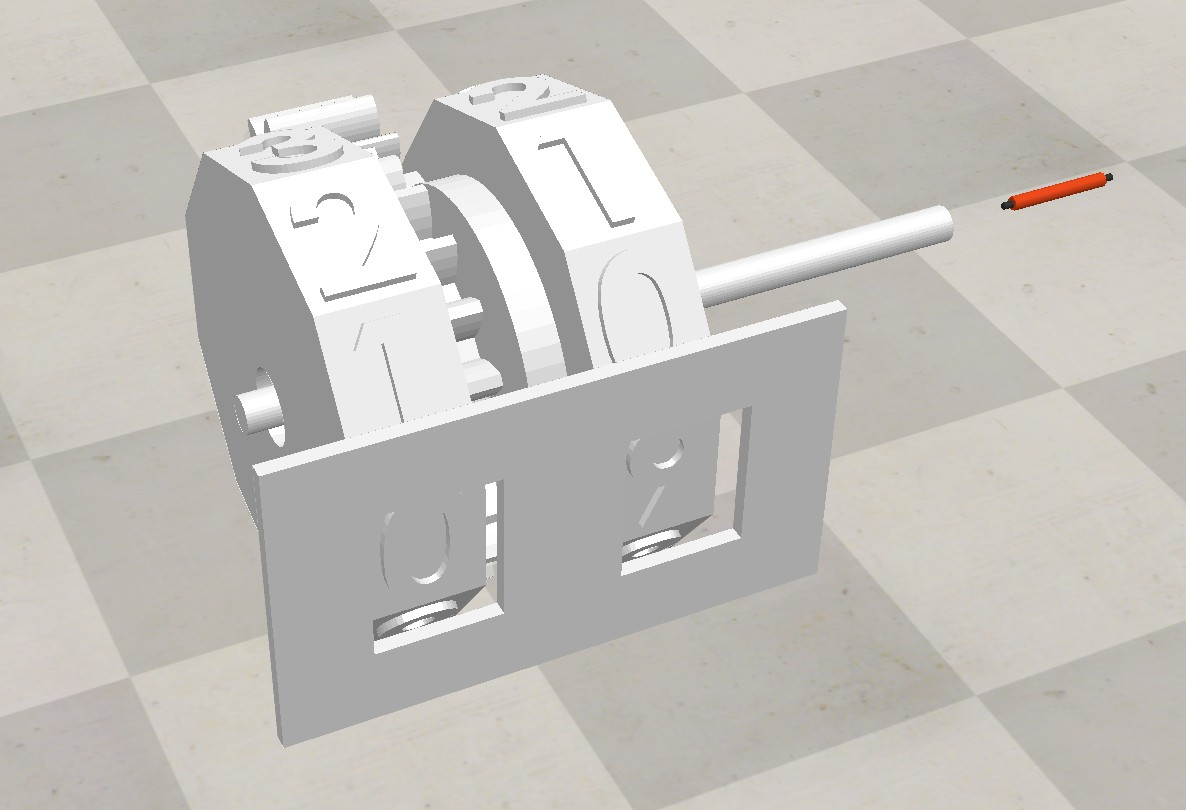
\includegraphics[width=13cm]{messageImage_1685927228163}
\caption{\Large 機械轉盤傳動計分系統}
\label{messageImage_1685927228163}
    
\section{製作過程}

模型是用SOLIDWORKS繪製,先將各個零件分別繪製,再依序組合完成,最後轉到CoppeliaSim預備模擬。數字輪盤的設計是將圓盤的曲面切割成數個平面並放上數字,齒輪則是經過相關數據的計算完成的,我們有再多製作一個面板使這個計分系統上的得分數更方便閱讀。\\
剛開始搜尋資料時很快就理解了它的運作原理,還認為計分板的繪製不太困難,實際下手畫圖才發現其實有很多細節需要注意,尤其是齒輪的嚙合需要更精細。其中遇到最大的瓶頸,是將SOLIDWORKS裡呼叫的標準零件放進組合圖容易自動跳回標準尺寸,以至於個位數齒輪的齒數繪製不易。且因尚未解決此問題,只能趁SOLIDWORKS檔還是我們所要的形狀時趕緊轉成stl檔到CoppeliaSim做程式設計。\\





\end{figure}


\chapter{程式碼}\

\section{球員控制程式}
 
 \begin{figure}[hbt!]
\begin{center}
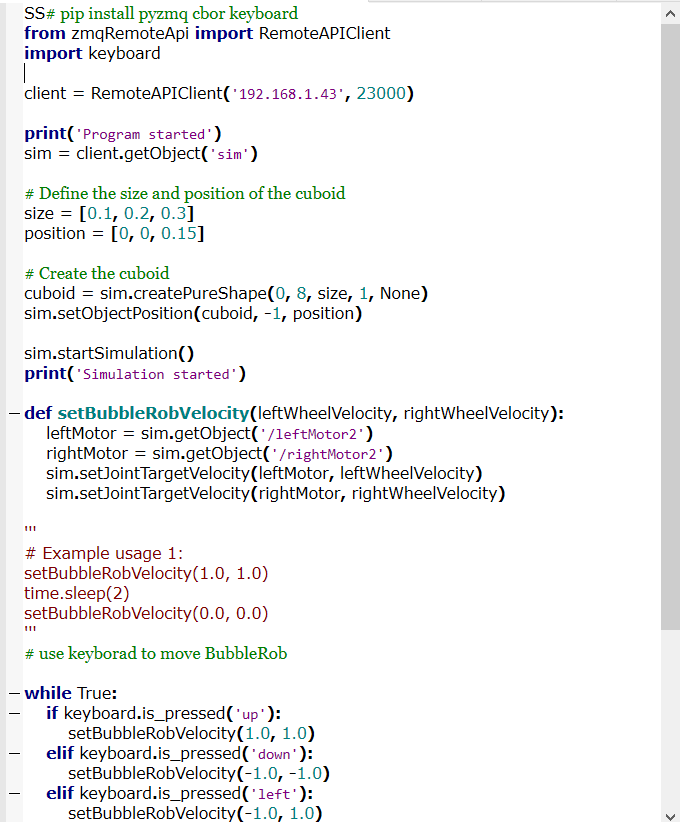
\includegraphics[width=10cm]{程式碼1}
\caption{\Large 球員控制程式碼}\label{fig.程式碼1}
\end{center}
\end{figure}

\begin{center}
 使用 RemoteAPIClient 來連接遠端的 API 服務器,以及使用keyboard 函式庫來控制鍵盤。\\
 \end{center}
 
\begin{figure}[hbt!]
\begin{center}
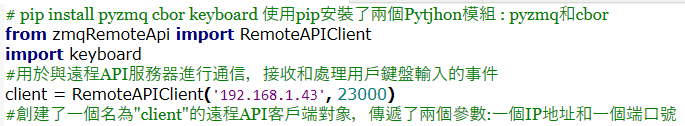
\includegraphics[width=13cm]{程式碼2}
\caption{\Large RemoteAPIClient}\label{fig.程式碼2}
\end{center}
\end{figure}

\newpage
 
\section{連線程序}

\begin{center}
主機的部分要先到小黑窗打指令ipconfig,搜尋本機位址
\end{center}

\begin{figure}[hbt!]
\begin{center}
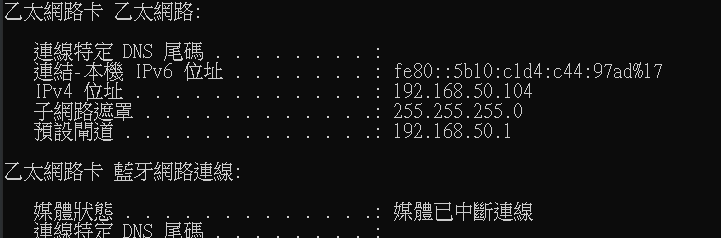
\includegraphics[width=12cm]{程式碼6}
\caption{\Large 查詢網路位址}\label{fig.程式碼6}
\end{center}
\end{figure}

\begin{center}
為了能在操控球員時能夠實時看到球場上的情況,所要做的前置作業
\end{center}

\begin{figure}[hbt!]
\begin{center}
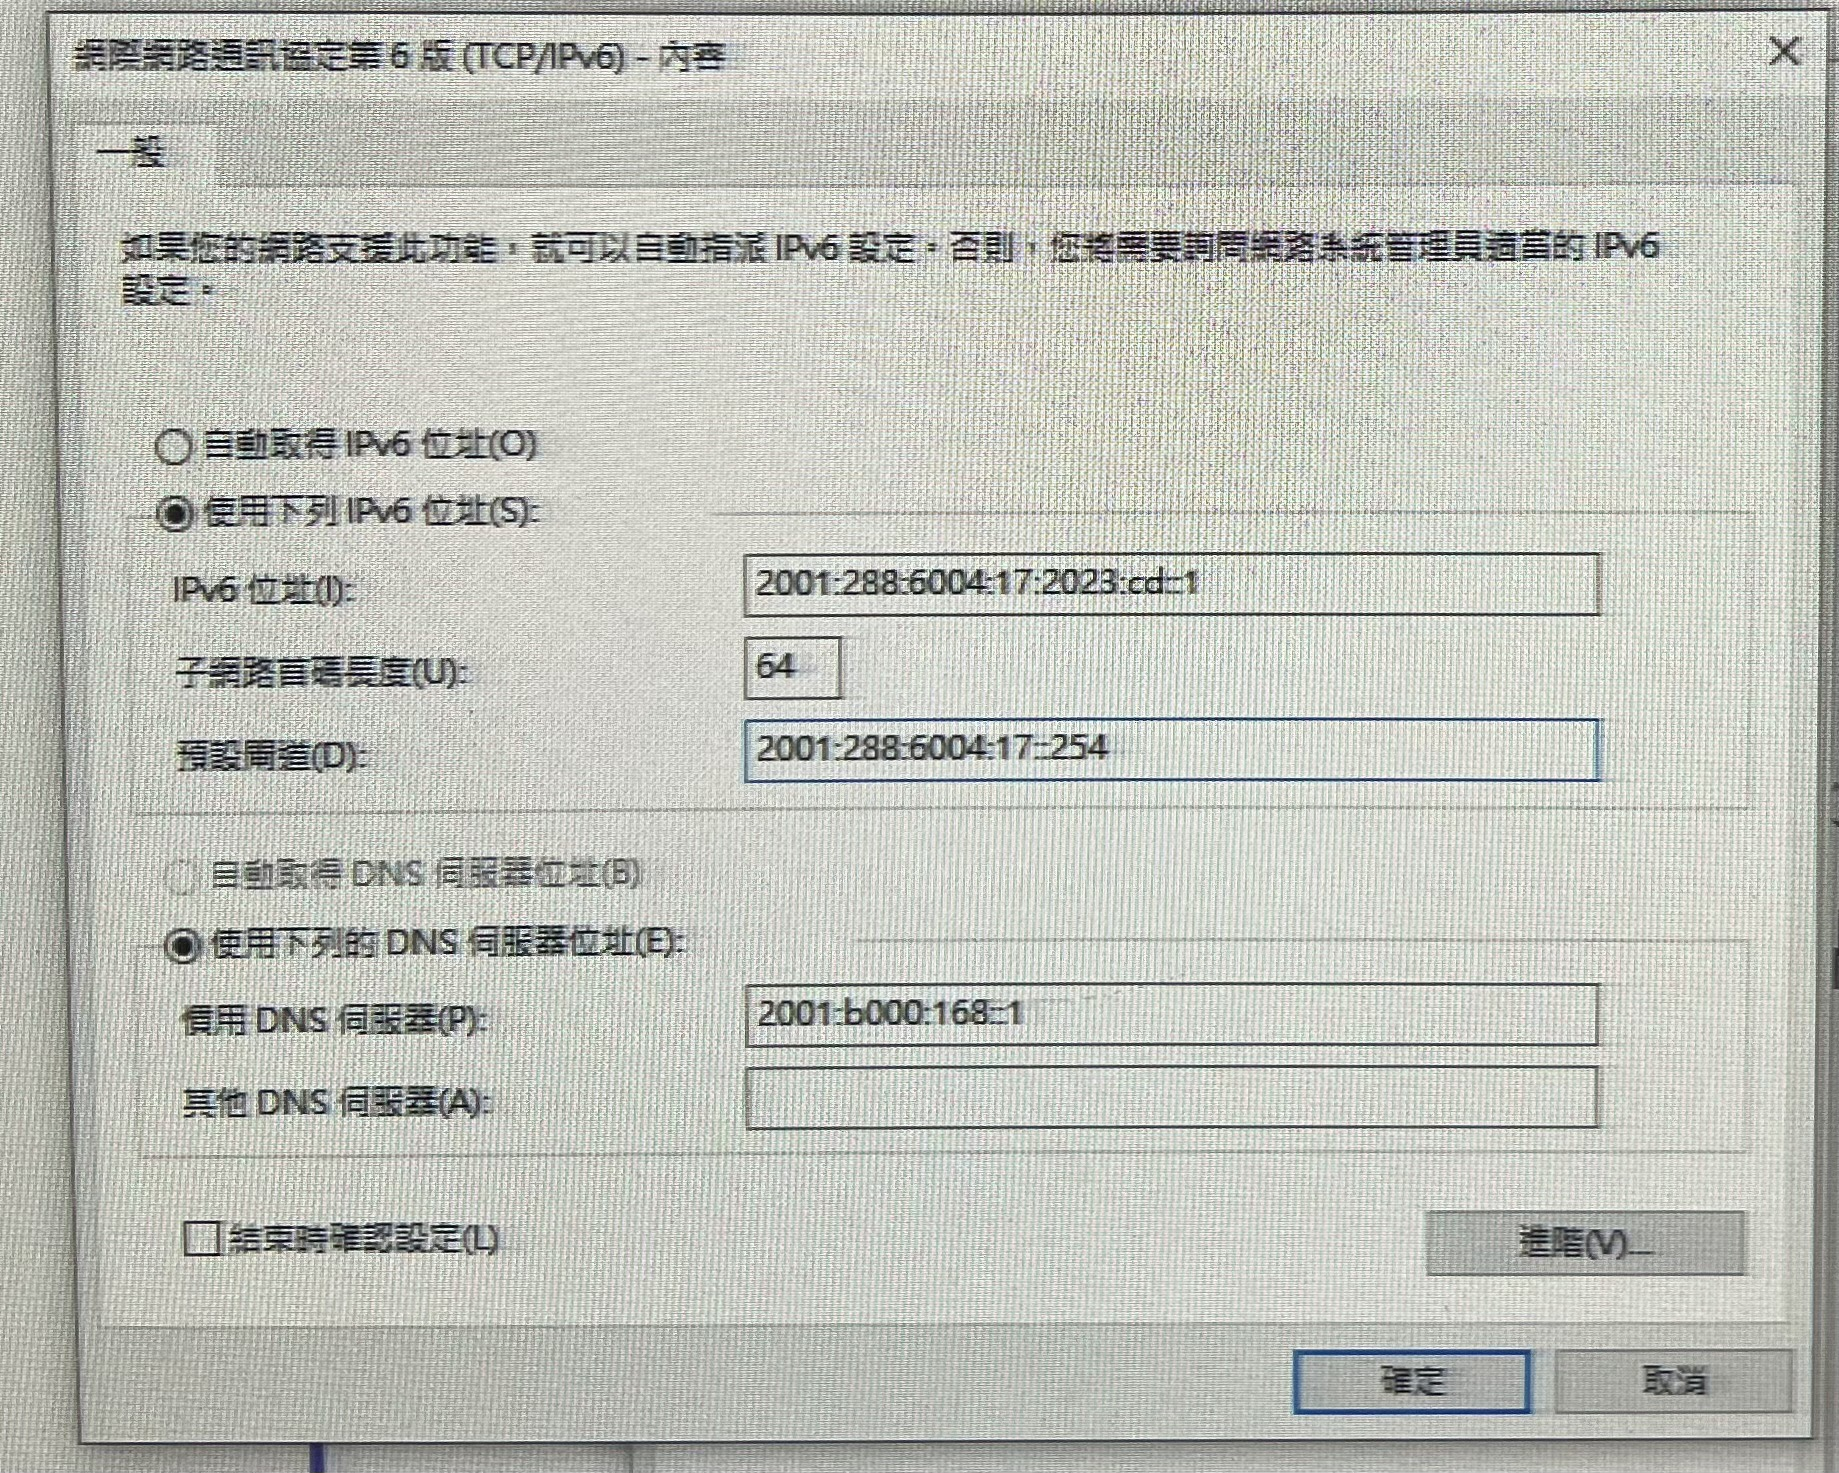
\includegraphics[width=10cm]{程式碼3}
\caption{\Large IPv6設置}\label{fig.程式碼3}
\end{center}
\end{figure}

\begin{center}
到防火牆進階設定裡面,新增規則,然後將規則類型改成連接埠
\end{center}

\begin{figure}[hbt!]
\begin{center}
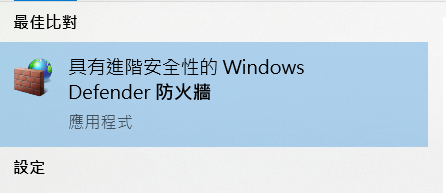
\includegraphics[width=10cm]{防火牆}
\caption{\Large 防火牆}\label{fig.防火牆}
\end{center}
\end{figure}

\begin{center}
將特定本機連接埠輸入23000至23050
\end{center}

\begin{figure}[hbt!]
\begin{center}
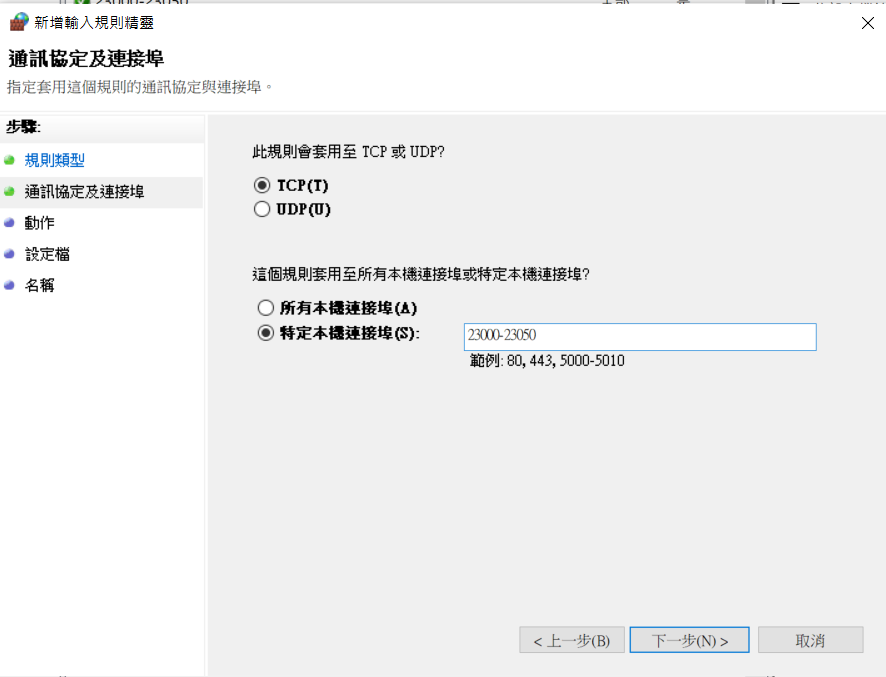
\includegraphics[width=10cm]{連接埠}
\caption{\Large 特定本機連接埠}\label{fig.連接埠}
\end{center}
\end{figure}

\begin{center}
下兩步為預設,到了名稱這裡打23000-23050
\end{center}

\begin{figure}[hbt!]
\begin{center}
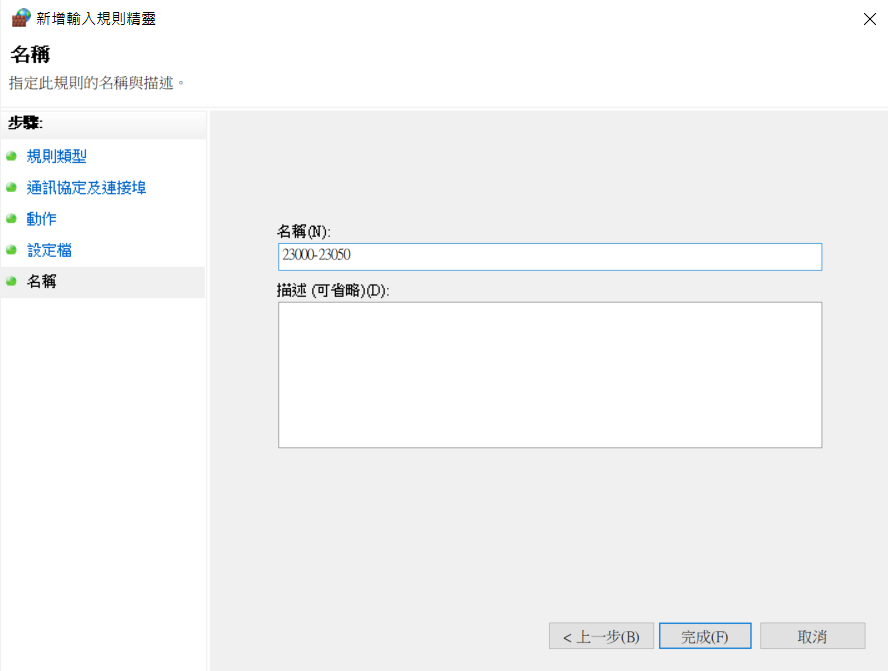
\includegraphics[width=10cm]{連接埠名稱}
\caption{\Large 連接埠名稱}\label{fig.連接埠名稱}
\end{center}
\end{figure}

\begin{figure}[hbt!]
\begin{center}
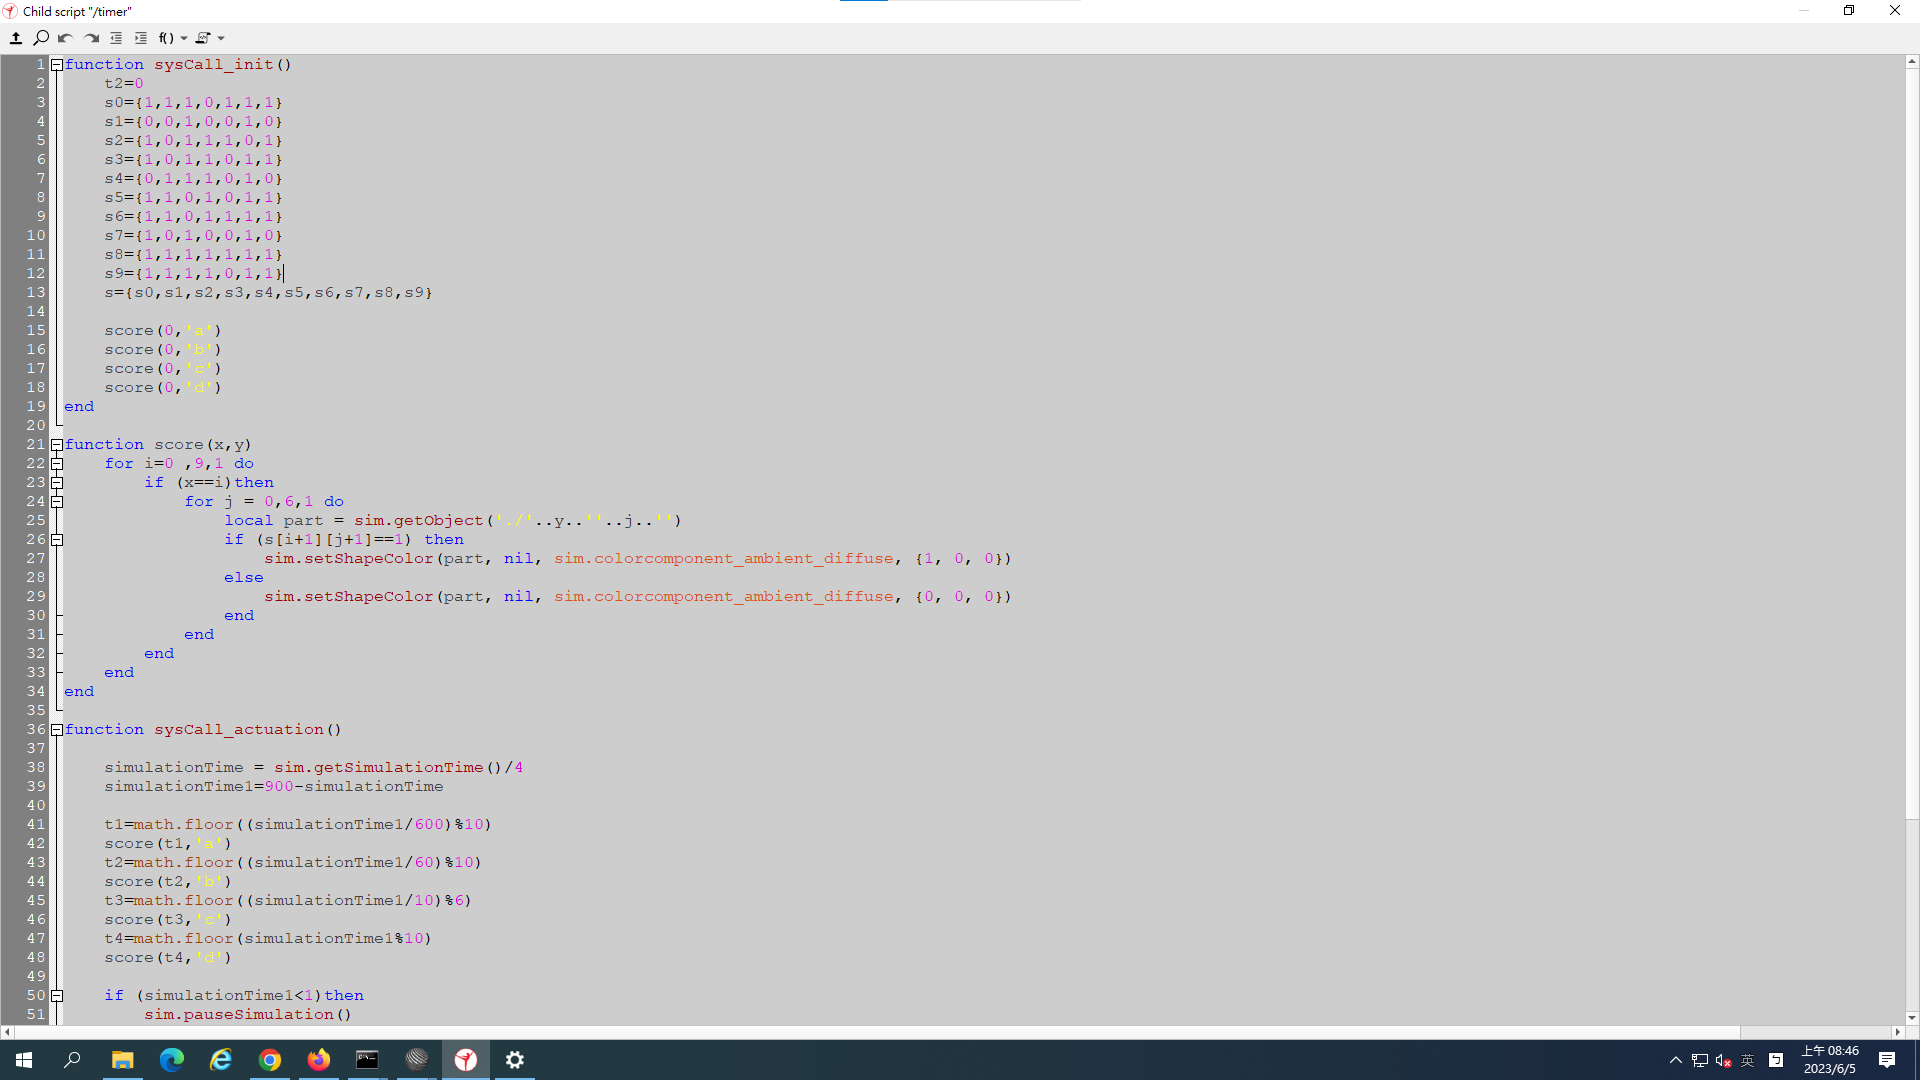
\includegraphics[width=20cm]{記分板程式碼}
\caption{\Large 記分板的程式碼}\label{fig.記分板程式碼}
\end{center}
\end{figure}
\newpage
\chapter{機器學習的訓練與模擬控制結果}
\section{訓練模型的基礎概念}
 訓練模型的原型是實體冰球機的機電系統,由於要訓練強化學習,所以需要將模型簡化至最簡潔的方式進行訓練,並取Open AI Gym的環境當作最簡化的訓練模型。由於強化學習是一種最佳化控制的方式,因此將Gym的Pong畫面當作輸入,輸出為擊錘移動方向,藉由調整當中的權重、偏差等參數,將參數調配到最優狀態。將可行的訓練方式套用到CoppeliaSim進行虛擬環境的訓練,並且可將訓練結果套用到實機進行運用。\\
\section{訓練模型的選用}
 利用Gym的環境訓練機器學習,以測試學習率、神經網路隱藏層的神經元個數、機器學習的啟動函數類型、訓練時影像大小等幾項參數與訓結果之間的關聯性,選用pyhton語言進行配置。剛開始我們運用Pygame模組來撰寫pong game的訓練環境,開始學習並了解Pygame的一些運用,嘗試建構出pong game場景(圖.\ref{fig.pong_pygame}),在基本功能編寫告一段落後,測試程式漏洞,發現對打時特定角度碰撞,球會超過擊錘的碰撞感測,導致出現球擊穿擊錘的現象。為了解決Pygame碰撞問題,做了幾種嘗試:修改Pygame的碰撞定義,更換碰撞感測的感測方式,問題依舊沒有顯著的改善,若增加過多的碰撞偵測點則會造成後續機器學習訓練時的運算負荷;另一種方法則是搭配pymunk的物理引擎模組使用(圖.\ref{fig.airhockey_pymunk}),使環境更符合實際物理現象,可加入碰撞、摩擦、力量大小、速度大小等可以個別設定和調用。當環境有了物理接下來就需要加入訓練所需的功能,如:訓練時的場景的即時影像畫面、即時獎勵回傳、該局結束時的場景重設和分數重置等功能。此時找到了Open AI Gym模組。\\
\begin{figure}[hbt!]
\begin{center}
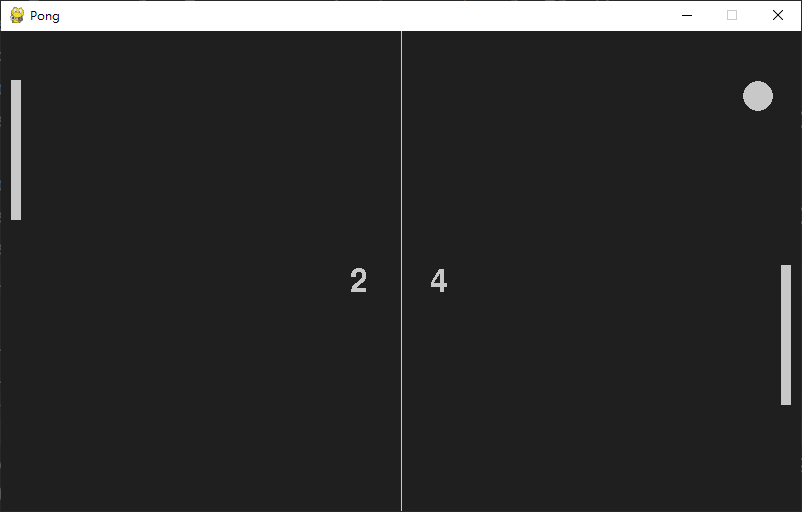
\includegraphics[width=12cm]{pong_pygame}
\caption{\Large Pygame模組編寫}
\label{fig.pong_pygame}
\end{center}
\end{figure}

\begin{figure}[hbt!]
\begin{center}
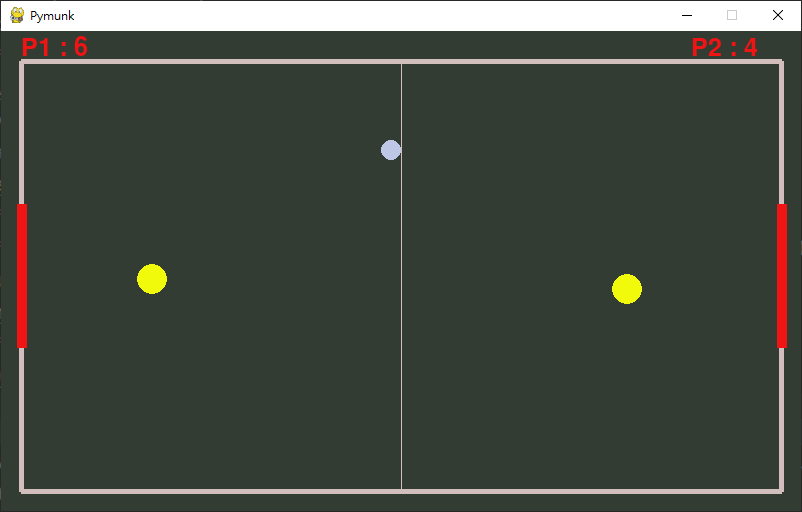
\includegraphics[width=12cm]{airhockey_pymunk}
\caption{\Large Pymunk模組編寫}
\label{fig.airhockey_pymunk}
\end{center}
\end{figure}
 \newpage %圖片空隙勿刪
 Open AI Gym裡面有十幾種訓練模型的環境,提供機器學習做訓練的環境。由於我們的訓練模型是pong game,在Gym模組裡面剛好有訓練模型,因此使用Gym模組相對於使用Pygame和pymunk的搭配來的方便,而且後續要在CoppeliaSim模擬環境模擬時也有套件可搭配使用,可簡化功能和訓練時所需的環境模型和訓練功能的程式編寫,另一方面自寫場景需要測試場景的漏洞,使用Gym可以節省檢查場景漏洞和修正的時間。\\
\section{訓練程式的運作}
 由於機器學習和影像處理需要大量的運算矩陣運算,因此如果只單獨透過Python本身運算比編譯語言執行的速度來的慢,所以使用Numpy程式庫來解決在Python環境矩陣運算速度慢的問題,以提升訓練機器學習時的運算效率。pickle是Python內部的序列化方式,主要是當機器學習訓練時可能因為一些原因需要暫時停止訓練,但為了讓已經停下的訓練再次重啟就需要透過pickle序列化的方式,將暫停前的訓練權重值透過pickle將其記錄下來,當訓練再次重啟時就可透過pickle.load讀取先前紀錄的pickle檔案就可回到當時暫停的狀態下繼續進行訓練。\\
 
 機器學習所運用的架構是強化學習並搭配神經網路來訓練機器學習,結合了強化學習不需要事先收集訓練資料、不需要特別教導,以及神經網路的非線性激活函數的計算和參數的記憶性。\\

\begin{figure}[hbt!]
\begin{center}
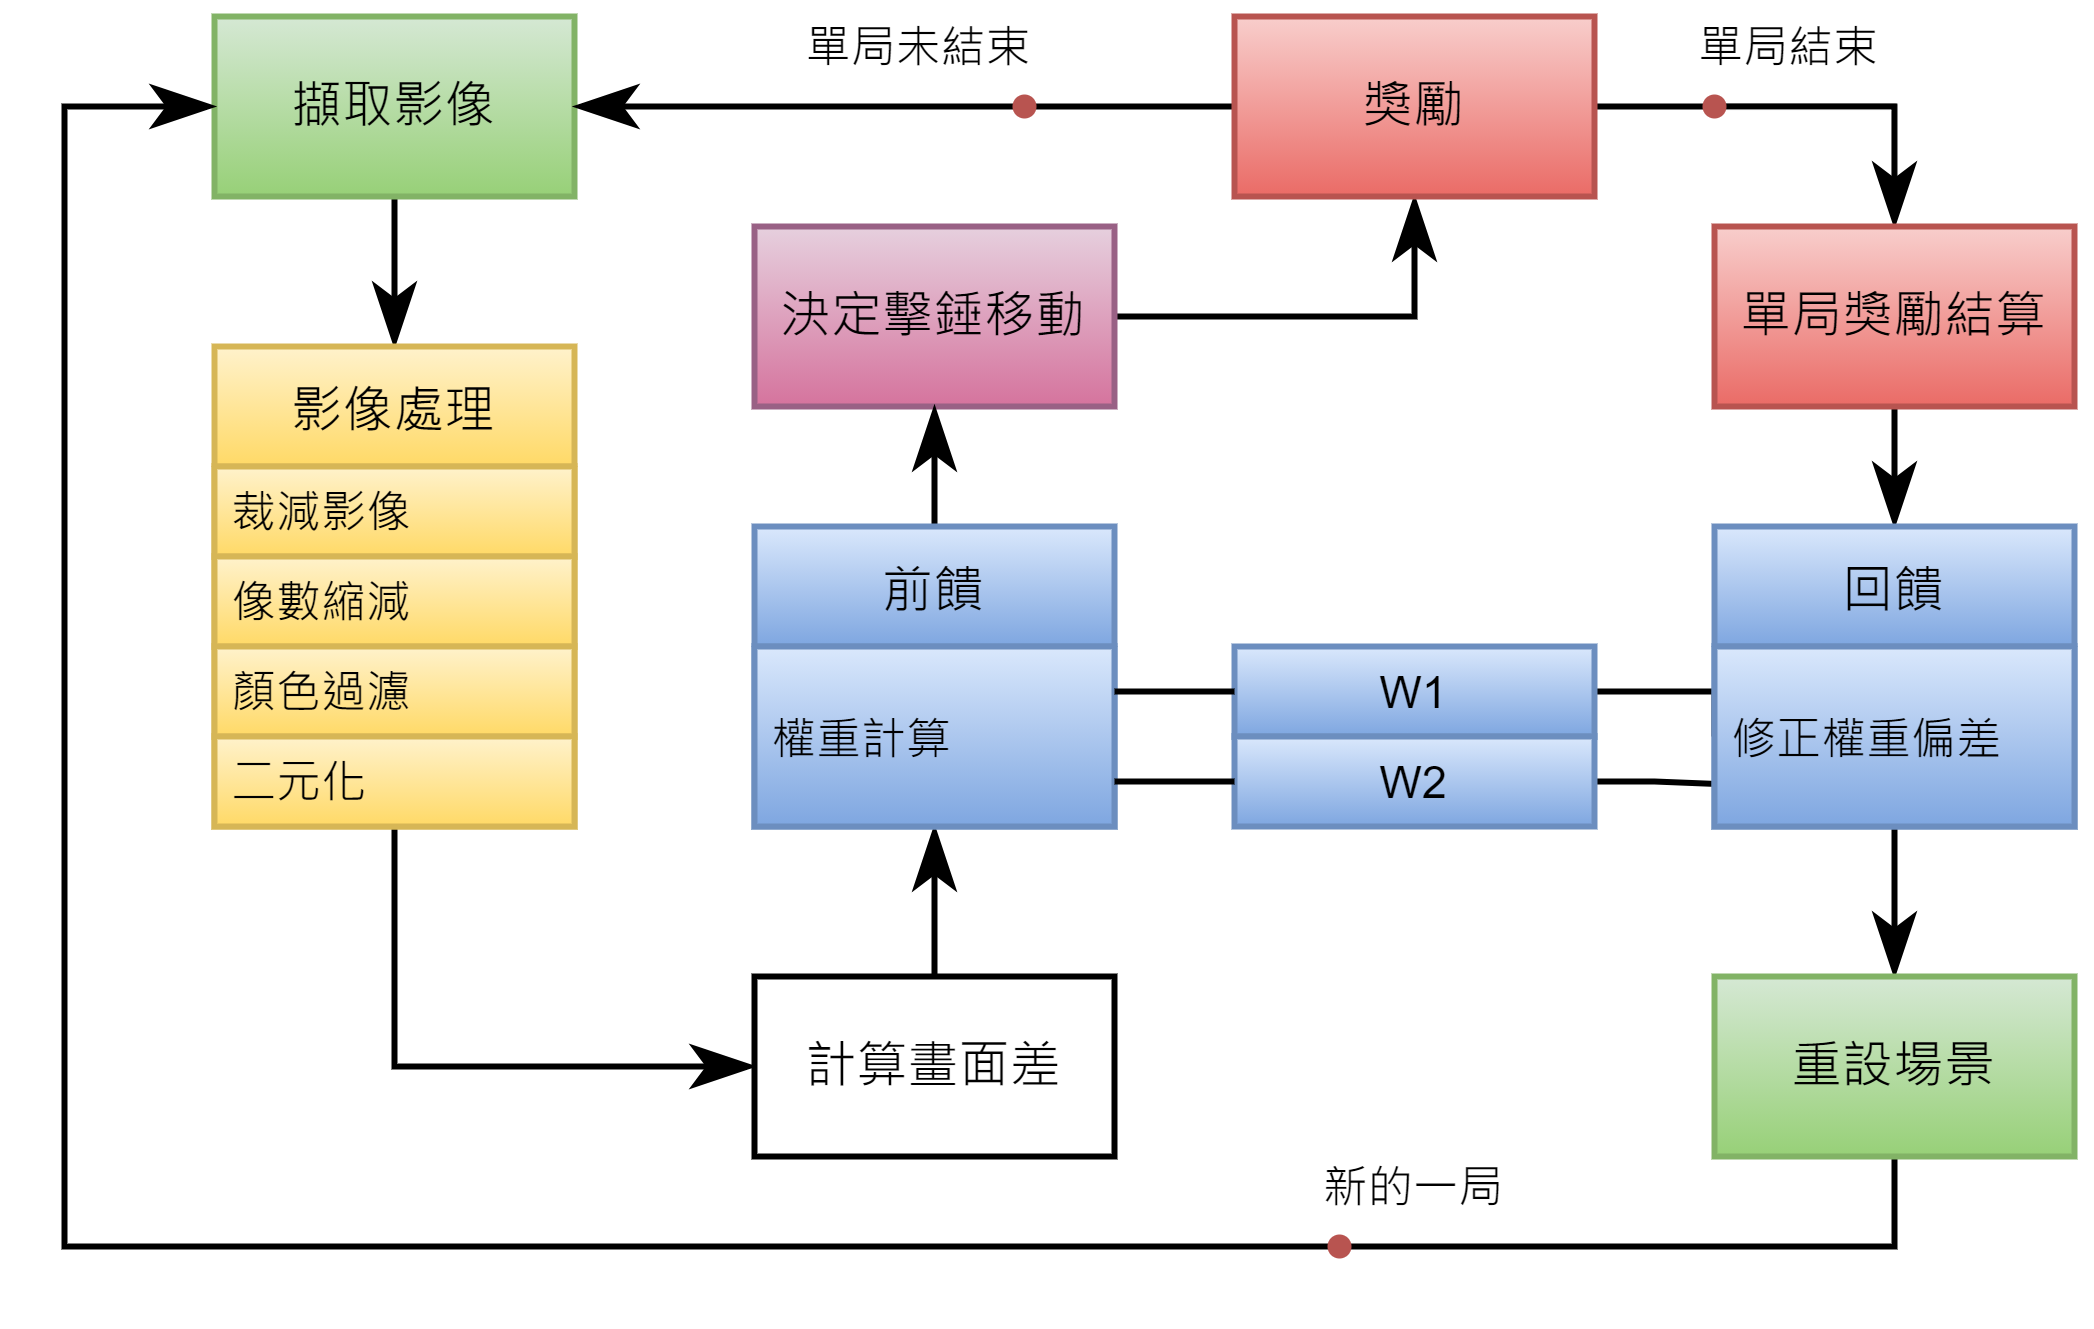
\includegraphics[width=15cm]{強化學習訓練流程}
\caption{\Large 強化學習訓練流程}
\label{fig.強化學習程式流程}
\end{center}
\end{figure}
%-----------------------------%

%=---------圖片空隙勿刪--------=%
%-----------------------------%
程式訓練流程(圖.\ref{fig.強化學習程式流程}):\\
 擷取影像,將影像裁剪至實際遊戲範圍,並簡化像素以利提高訓練時的計算速度,減少運算時的負擔,過濾顏色只保留球與擊錘,並把取到的影像二元化,取兩幀畫面進行比較,掌握球與擊錘間的相對位置(畫面差),透過前饋:計算球在環境的狀態及擊錘移動的決策,畫面差透過W1權重來計算球在環境的狀態,透過W2權重並經過啟動函數(activation function)得出擊錘移動的決策。透過產生隨機值的方式來與擊錘移動決策值進行比較,判定隨機值落在的區間來決定移動策略。計算discount reward及獎勵的加總。獎勵設定球若超過了對手,獎勵為+1;如果錯過球,則獎勵為-1;其餘狀態獎勵為0。\\

 在單局結束時,紀錄下該局累積下來的經驗,亦是紀錄該局所修正出來的參數而進行獎勵計算、log probability、RMSprop優化率減因子和反饋(back propagation),當訓練次數到達指定次數會以pickle做紀錄,存下的數據可再次導入模型進行實際運用,或是當程式中斷後可重新匯入進行訓練。比較持續訓練與中斷後重新匯入訓練的差異,測試算法版本為Pong2,MSE代表均方誤差值,pong2\_ r表示中斷後重新匯入的訓練數據,pong2與pong2\_ r標示個別表示該訓練每局分數的紀錄,pong2 MSE與pong2\_ r MSE標示個別表示該訓練均方誤差值紀錄(圖.\ref{fig.比較中斷數據}) \\
\begin{figure}[hbt!]
\begin{center}
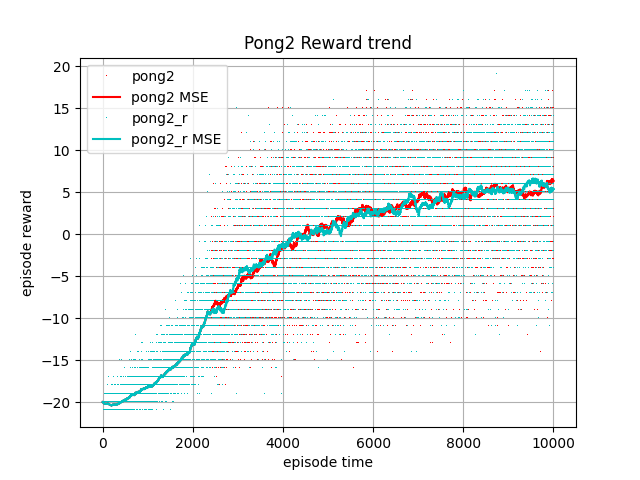
\includegraphics[width=15cm]{pong2_RvsNR}
\caption{\Large 比較中斷後訓練差異}
\label{fig.比較中斷數據}
\end{center}
\end{figure}

\section{訓練算法與參數比較}
 pong1版本是karpathy的pg\- pong.py的原始碼[\ref{R.pong1}],pong1.1原始碼則是schinger的pong\_ actor\- critic/pg\- pong\- ac.py[\ref{R.pong1.1}],pong1.2的是修改pong1的學習率參數從0.001調整到0.0001,並且將裁切後80*80的影像改成75*80。pong2版本是etienne87的pg\- pong.py的原始碼[\ref{R.pong2}]修改的,將動作策略由上下上替換成停上下的模式,學習率也配合調整,由0.0001調至0.001。\\
 
 下圖(圖.\ref{fig.比較中斷數據})為這幾個版本的訓練趨勢的紀錄提供做比較,訓練次數(圖.\ref{fig.比較中斷數據}之水平軸)為3000局做比較,小點為每局積分總和(圖.\ref{fig.比較中斷數據}之垂直軸),線條為累積積分的均方誤差值,積分計算$-21$分代表對面得21分,即機器訓練所得分數-對面所得分數。訓練存在隨機性(Stochastic),因此每次訓練所得趨勢會有所差異。\\
\begin{table}[hbt!]
\center\large
\setlength{\tabcolsep}{0.75cm}{
\begin{tabular}{|c|c|c|c|}
\hline  版本名稱 & 標示顏色 & 啟動函數 & 參考來源\\
\hline  pong1 &  紅色 & sigmoid & [\ref{R.pong1}]\\
\hline  pong1.1 &  藍色 & sigmoid & [\ref{R.pong1.1}]\\
\hline  pong1.2 &  橘色 & sigmoid & [\ref{R.pong1}]\\
\hline  pong2 & 綠色 & softmax & [\ref{R.pong2}] \\
\hline
\end{tabular}}
\caption{\Large 版本標示}
\end{table}

\begin{figure}[hbt!]
\begin{center}
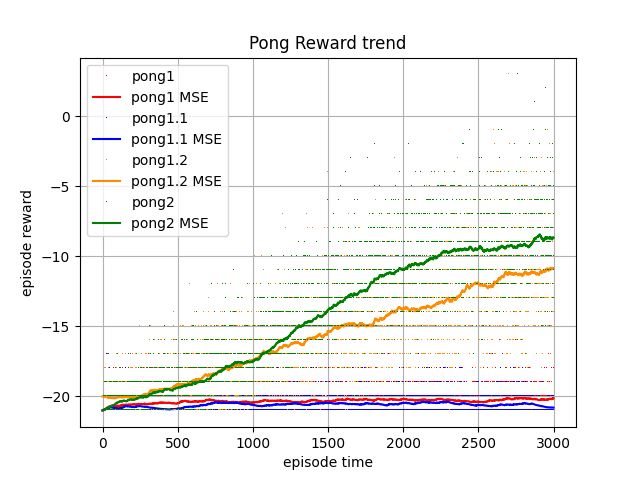
\includegraphics[width=15cm]{pong}
\caption{\Large 各版本差異}
\label{fig.各版本差異}
\end{center}
\end{figure}
觀察後發現,pong2版本的訓練結果得分最高,pong1.2的訓練結果為次高,pong1及pong1.1的版本沒有收斂,訓練對打的表現沒有進步的跡象,參數還需做調整及測試,pong2及pong1.2為主要選擇訓練演算法。接下來測試pong1的學習率調整成0.0001,pong1.2的學習率上調到0.001,以pong2版本當作對照(圖.\ref{fig.比較中斷數據}),同樣以3000次訓練當作參考依據,測試結果三者相當接近。因為訓練時間及設備限制,修正後的pong1與pong1.2版本所以擇一與pong2進行長時間訓練比較,因此選用pong1.2版本。

\begin{figure}[hbt!]
\begin{center}
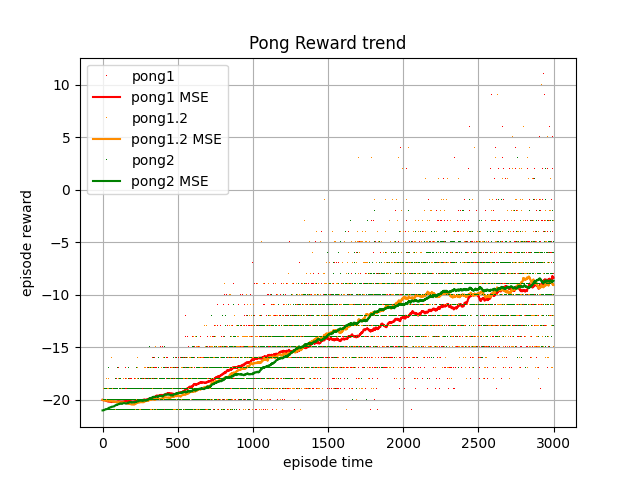
\includegraphics[width=15cm]{pong_test}
\caption{\Large pong1與1.2調整後數據比較}
\label{fig.調整後數據比較}
\end{center}
\end{figure}

\begin{flushleft}
電腦規格:\\
\end{flushleft}
\begin{enumerate}[1.]
\item 研究室桌上型電腦(長時間訓練所使用):\\
Windows10 專業版 2004\\
CPU:Intel i7-7700 3.60GHZ\\
RAM:16GB\\
GPU:NVDIA GTX1050
\item 個人筆記型電腦(3000次訓練數據為此設備訓練,短時間測試用):
Windows10 家用版 2004\\
CPU:Intel i7-8750H 2.20GHZ\\
RAM:8GB\\
GPU:NVDIA GTX1050 Ti\\

總訓練時數約336\textasciitilde 350小時(圖.\ref{fig.pong2與pong1.2長時間訓練比較}),pong2的數據均方誤差(MSE)數據較穩定,由於訓練中無法得知當下是處於數據波動的較優或較差的狀態,若要中斷訓練則有可能剛好處於波動的較差的狀態,因此選擇pong2的版本當作訓練算法較為穩定。
\end{enumerate}
\begin{figure}[hbt!]
\begin{center}
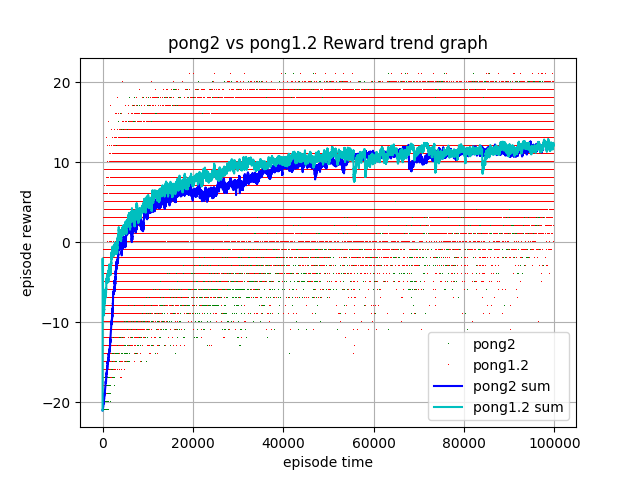
\includegraphics[width=15cm]{pong2_vs_pong1.2_reward}
\caption{\Large pong2與pong1.2長時間訓練數據}
\label{fig.pong2與pong1.2長時間訓練比較}
\end{center}
\end{figure}



\section{CoppeliaSim RemoteAPI}
在進行強化學習時主要是透過CoppeliaSim中的Remote API 函數來取得模擬場景中所需要的資訊,並在進行訓練後再回傳到CoppeloaSim做控制的動作。\\
\subsection{Remote API模組及動態連結函示庫}
在啟用RemoteAPI需要先準備以下三項模組和動態連結函示庫,並將此三項與預執行的程式放在同一目錄下:
\begin{itemize}
\item sim.py
\item simConst.py
\item remoteApi.dll、remoteApi.dylib 或 remoteApi.so (依序適用於:Windows、MacOS、Ubuntu)
\end{itemize}
sim.py及simConst.py為Python模組,其位於:\\
CoppeliaSim安裝目錄$\backslash$programming$\backslash$remoteApiBindings$\backslash$python$\backslash$python\\
remoteApi.dll為RemoteAPI動態連結函示庫,其位於:\\
CoppeliaSim安裝目錄$\backslash$programming$\backslash$remoteApiBindings$\backslash$lib$\backslash$lib$\backslash$作業系統\\
\subsection{Remote API埠使用}
Remote API是通過通訊埠取得環境資訊,在CoppeliaSim中預設埠號為19997,只有預設埠不需開啟特定場景就可進行通訊並控制所有功能,且在大量影像資料處理時可啟用多埠,使其中一個通訊埠用於影像處理,另一個則用於控制,新增的通訊埠需在安裝資料夾中的remoteApiConnections.txt加入需要的埠號。\\
\section{Open AI Gym自定義環境}
Open AI Gym可以支持我們以自己搭建的環境進行訓練,因此我們透過Gym並以CoppeliaSim虛擬環境中搭建的冰球機模型來完成訓練,而Gym所使用的環境參數就是由前述的Remote API來取得。Gym將環境抽象為一個類別(class)在該類別(class)中需分別定義以下參數來達成自定義環境的訓練。\\

\begin{enumerate}
\item init:初始化CoppeliaSim中的環境參數。
\item seed:用於設置環境變數。
\item make observation :用於設置環境場景中需觀察的值,如:擊錘位置、冰球位置...等。
\item make action:設置擊錘的移動速度。
\item step:訓練的主要邏輯,如:遊戲是否結束、reward函數返回值、環境觀察值...等。
\item reset:將環境重置。
\item render:可搭配OpenCV進行數據渲染。
\item close:釋放環境數據。\\
\end{enumerate}

\section{總結}
選擇適合的演算法,並找到適合的參數,透過訓練提升機器對打的能力,訓練的時間越長,學習對打的成效越好,但訓練後期進步的幅度趨緩,因此得評估訓練的時間長度以符合整體效益。在模擬環境中利用RemoteAPI建置了跨平台控制,並運用CoppeliaSim中視覺傳感器所取得之影像透過OpenCV加以處理便於輔助玩家進行對打,在程式中則使用OpenCV處理及簡化過的影像進行擊錘移動的計算,將計算後得出的結果回傳到CoppeliaSim中的環境,使擊錘做出對應的動作。
\newpage

%=---------------附錄-----------------=%
\addcontentsline{toc}{chapter}{附錄} %新增目錄名稱
\begin{appendix}
\renewcommand{\thesection}{\bf 附錄 \Alph{section}}%設定標題名稱
\begin{center}
\fontsize{20pt}{0em}\selectfont\bf 附錄
\end{center}
\section*{LaTeX}
LaTex 為一種程式語言,支援標準庫 (Standard Libraries) 和外部程式庫 (External Libraries),不過與一般程式語言不同的是,它可以直接表述 Tex 排版結構,類似於 PHP 之於 HTML 的概念。但是直接撰寫 LaTex 仍較複雜,因此可以藉由 Markdown 這種輕量的標註式語言先行完成文章,再交由 LaTex 排版。
此專題報告採用編輯軟體為LaTeX,綜合對比Word編輯方法,LaTeX較為精準正確、更改、製作公式等,以便符合規範、製作。
 \begin{table}[htbp] %htbp代表表格浮動位置
			\centering%表格居中
			\caption{文字編輯軟體比較表}%表:標題
			\large%字體大小
			\label{tab_文字編輯軟體比較表:scale}
			\begin{tabular}{|c|c|c|c|c|c|c|}
			\hline
			\diagbox[width=8em]& 相容性 & 直觀性 & 文件排版 & 數學公式 & 微調細部\\ 
			\hline
			LaTeX 		&$\surd$&		&$\surd$&$\surd$&$\surd$\\
			\hline
			Word	 	&		&$\surd$&		&		&$\surd$\\
			\hline
			
			\end{tabular}
		\end{table}	
\newpage
\begin{itemize} 
\item 特點:
\end{itemize}
\begin{enumerate}
\item 相容性:以Word為例會有版本差異,使用較高版本編輯的文件可能無法以較低的版本開啟,且不同作業系統也有些許差異;相比LaTeX可以利用不同編譯器進行編譯,且為免費軟體也可移植至可攜系統內,可以搭配Github協同編譯。
\item 文件排版:許多規範都會要求使用特定版型,使用文字編譯環境較能準確符合規定之版型,且能夠大範圍的自定義排定所需格式,並能不受之後更改而整體格式變形。
\item 數學公式呈現:LaTex可以直接利用本身多元的模組套件加入、編輯數學公式,在數學推導過程能夠快速的輸入自己需要的內容即可。
\item 細部調整:在大型論文、報告中有多項文字、圖片、表格,需要調整細部時,要在好幾頁中找尋,而LaTeX可以分段章節進行編譯,再進行合併處理大章節。
\end{enumerate}
\end{appendix}
\section*{FFmpeg}
FFmpeg是一個開放原始碼的自由軟體,可以對音訊和視訊進行多種格式的錄影、轉檔、串流功能。在專題訓練過程中透過FFmpeg的視訊錄製的功能記錄對打影像來了解實際訓練狀況。
\newpage
\newpage
%=-------------作者簡介-----------------=%
    \addcontentsline{toc}{chapter}{作者簡介}
    \begin{center}
	\fontsize{20pt}{0em}\selectfont \bf{作者簡介}\\
	\end{center}	
	{\begin{textblock}{6}(0,0.5)
	\begin{figure}
	
\includegraphics[width=1.25in]{member1}  %作者照片
	\end{figure}
	\end{textblock}}
	{\renewcommand\baselinestretch{0.99}\selectfont %設定以下行距
	{\begin{textblock}{15}(3.5,0.7)%{寬度}(以左上角為原點之右移量,下移量)
	\noindent\fontsize{14pt}{0em}\selectfont \makebox[4em][s]{姓名}\enspace:\enspace
    \fontsize{14pt}{0em}\selectfont \makebox[4em][s]{張韋翔}\\     \hspace*{\fill} \\
    \fontsize{14pt}{0em}\selectfont \makebox[4em][s]{學號}\enspace:\enspace
    \fontsize{14pt}{0em}\selectfont \makebox[4em][s]{41023154} \\ %\makebox為文本盒子
    \hspace*{\fill} \\
    \fontsize{14pt}{0em}\selectfont \makebox[4em][s]{畢業學校}\enspace:\enspace
    \fontsize{14pt}{0em}\selectfont \makebox[9em][s]{國立員林農工}\\
    \fontsize{14pt}{0em}\selectfont \makebox[5em][s]{\quad}\enspace\enspace
    \fontsize{14pt}{0em}\selectfont \makebox[8em][s]{機械科}\\
    \end{textblock}}}
   % \hspace*{\fill} \\
   \vspace{2em}
	{\begin{textblock}{6}(0,2.3)
	\begin{figure}
	
\includegraphics[width=1.15in]{member1}  %作者照片
    \end{figure}
    \end{textblock}}
    {\renewcommand\baselinestretch{0.99}
    \selectfont %設定以下行距
    {\begin{textblock}{15}(3.5,2.5) %{寬度}(以左上角為原點之右移量,下移量)
\noindent\fontsize{14pt}{0em}\selectfont \makebox[4em][s]{姓名}\enspace:\enspace
\fontsize{14pt}{0em}\selectfont \makebox[4em][s]{林政蔚}\\ 
\hspace*{\fill} \\
\fontsize{14pt}{0em}\selectfont \makebox[4em][s]{學號}\enspace:\enspace
\noindent\fontsize{14pt}{0em}\selectfont \makebox[4em][s]{41023135} \\ 
\hspace*{\fill} \\
\fontsize{14pt}{0em}\selectfont \makebox[4em][s]{畢業學校}\enspace:\enspace
\fontsize{14pt}{0em}\selectfont \makebox[9em][s]{國立台中高工}\\
\fontsize{14pt}{0em}\selectfont \makebox[5em][s]{\quad}\enspace\enspace
\fontsize{14pt}{0em}\selectfont \makebox[8em][s]{機械科}\\
    \end{textblock}}}
    %\hspace*{\fill} \\
    \vspace{2em}
    {\begin{textblock}{6}(0,4.1)
    \begin{figure}
        
\includegraphics[width=1.15in]{member1} %{}內是圖片文件的相對路徑
    \end{figure}
    \end{textblock}}
    {\renewcommand\baselinestretch{0.99}\selectfont %設定以下行距
    {\begin{textblock}{15}(3.5,4.3) %{寬度}(以左上角為原點之右移量,下移量)
\noindent\fontsize{14pt}{0em}\selectfont \makebox[4em][s]{姓名}\enspace:\enspace%\noindent指定首行不進行縮排
\fontsize{14pt}{0em}\selectfont \makebox[4em][s]{邱仲陞}\\ 
\hspace*{\fill} \\
\noindent\fontsize{14pt}{0em}\selectfont \makebox[4em][s]{學號}\enspace:\enspace
\noindent\fontsize{14pt}{0em}\selectfont \makebox[4em][s]{41023140} \\ %\makebox為文本盒子
\hspace*{\fill} \\
\noindent\fontsize{14pt}{0em}\selectfont \makebox[4em][s]{畢業學校}\enspace:\enspace
\noindent\fontsize{14pt}{0em}\selectfont \makebox[9em][s]{市立大甲高工}\\
\noindent\fontsize{14pt}{0em}\selectfont \makebox[5em][s]{\quad}\enspace\enspace
\noindent\fontsize{14pt}{0em}\selectfont \makebox[8em][s]{製圖科}\\
    \end{textblock}}}
   % \hspace*{\fill} \\
   \vspace{2em}
    {\begin{textblock}{6}(0,5.9)
    \begin{figure}
        
\includegraphics[width=1.15in]{member1} %{}內是圖片文件的相對路徑
    \end{figure}
    \end{textblock}}
    {\renewcommand\baselinestretch{0.99}\selectfont %設定以下行距
    {\begin{textblock}{15}(3.5,6.1) %{寬度}(以左上角為原點之右移量,下移量)
\noindent\noindent\fontsize{14pt}{0em}\selectfont \makebox[4em][s]{姓名}\enspace:\enspace
\noindent\fontsize{14pt}{0em}\selectfont \makebox[4em][s]{林建三}\\ \hspace*{\fill} \\
\noindent\fontsize{14pt}{0em}\selectfont \makebox[4em][s]{學號}\enspace:\enspace
\noindent\fontsize{14pt}{0em}\selectfont \makebox[4em][s]{41023133} \\ \hspace*{\fill} \\
\noindent\fontsize{14pt}{0em}\selectfont \makebox[4em][s]{畢業學校}\enspace:\enspace
\noindent\fontsize{14pt}{0em}\selectfont \makebox[9em][s]{市立大甲高工}\\
\noindent\fontsize{14pt}{0em}\selectfont \makebox[5em][s]{\quad}\enspace\enspace
\noindent\fontsize{14pt}{0em}\selectfont \makebox[8em][s]{製圖科}\\
    \end{textblock}}}
    %\hspace*{\fill} \\
\vspace{2em}
    {\begin{textblock}{6}(0,7.7)
    \begin{figure}
        
\includegraphics[width=1.15in]{member2} %{}內是圖片文件的相對路徑
    \end{figure}
    \end{textblock}}
    \renewcommand\baselinestretch{0.99}\selectfont %設定以下行距
    {\begin{textblock}{15}(3.5,7.9) %{寬度}(以左上角為原點之右移量,下移量)
	\noindent\noindent\fontsize{14pt}{0em}\selectfont \makebox[4em][s]{姓名}\enspace:\enspace
	\noindent\fontsize{14pt}{0em}\selectfont \makebox[4em][s]{李宛妮}\\ \hspace*{\fill} \\
	\noindent\fontsize{14pt}{0em}\selectfont \makebox[4em][s]{學號}\enspace:\enspace
	\noindent\fontsize{14pt}{0em}\selectfont \makebox[4em][s]{41023105} \\ \hspace*{\fill} \\
	\noindent\fontsize{14pt}{0em}\selectfont \makebox[4em][s]{畢業學校}\enspace:\enspace
	\noindent\fontsize{14pt}{0em}\selectfont \makebox[9em][s]{國立斗南高中}\\
	\noindent\fontsize{14pt}{0em}\selectfont \makebox[5em][s]{\quad}\enspace\enspace
	\noindent\fontsize{14pt}{0em}\selectfont \makebox[8em][s]{普通科}\\
    \end{textblock}}
\newpage
    \addcontentsline{toc}{chapter}{作者簡介}
    \begin{center}
	\fontsize{20pt}{0em}\selectfont \bf{作者簡介}\\
	\end{center}	
	{\begin{textblock}{6}(0,0.5)
	\begin{figure}
	
\includegraphics[width=1.25in]{member2}  %作者照片
	\end{figure}
	\end{textblock}}
	{\renewcommand\baselinestretch{0.99}\selectfont %設定以下行距
	{\begin{textblock}{15}(3.5,0.7)%{寬度}(以左上角為原點之右移量,下移量)
	\noindent\fontsize{14pt}{0em}\selectfont \makebox[4em][s]{姓名}\enspace:\enspace
    \fontsize{14pt}{0em}\selectfont \makebox[4em][s]{林廷芸}\\     \hspace*{\fill} \\
    \fontsize{14pt}{0em}\selectfont \makebox[4em][s]{學號}\enspace:\enspace
    \fontsize{14pt}{0em}\selectfont \makebox[4em][s]{41023107} \\ %\makebox為文本盒子
    \hspace*{\fill} \\
    \fontsize{14pt}{0em}\selectfont \makebox[4em][s]{畢業學校}\enspace:\enspace
    \fontsize{14pt}{0em}\selectfont \makebox[9em][s]{市立新北高工}\\
    \fontsize{14pt}{0em}\selectfont \makebox[5em][s]{\quad}\enspace\enspace
    \fontsize{14pt}{0em}\selectfont \makebox[8em][s]{製圖科}\\
    \end{textblock}}}
   % \hspace*{\fill} \\
   \vspace{2em}
	{\begin{textblock}{6}(0,2.3)
	\begin{figure}
	
\includegraphics[width=1.15in]{member2}  %作者照片
    \end{figure}
    \end{textblock}}
    {\renewcommand\baselinestretch{0.99}
    \selectfont %設定以下行距
    {\begin{textblock}{15}(3.5,2.5) %{寬度}(以左上角為原點之右移量,下移量)
\noindent\fontsize{14pt}{0em}\selectfont \makebox[4em][s]{姓名}\enspace:\enspace
\fontsize{14pt}{0em}\selectfont \makebox[4em][s]{王郁淳}\\ 
\hspace*{\fill} \\
\fontsize{14pt}{0em}\selectfont \makebox[4em][s]{學號}\enspace:\enspace
\noindent\fontsize{14pt}{0em}\selectfont \makebox[4em][s]{41023102} \\ 
\hspace*{\fill} \\
\fontsize{14pt}{0em}\selectfont \makebox[4em][s]{畢業學校}\enspace:\enspace
\fontsize{14pt}{0em}\selectfont \makebox[9em][s]{市立新北高工}\\
\fontsize{14pt}{0em}\selectfont \makebox[5em][s]{\quad}\enspace\enspace
\fontsize{14pt}{0em}\selectfont \makebox[8em][s]{製圖科}\\
    \end{textblock}}}
    %\hspace*{\fill} \\
    \vspace{2em}
    {\begin{textblock}{6}(0,4.1)
    \begin{figure}
        
\includegraphics[width=1.15in]{member2} %{}內是圖片文件的相對路徑
    \end{figure}
    \end{textblock}}
    {\renewcommand\baselinestretch{0.99}\selectfont %設定以下行距
    {\begin{textblock}{15}(3.5,4.3) %{寬度}(以左上角為原點之右移量,下移量)
\noindent\fontsize{14pt}{0em}\selectfont \makebox[4em][s]{姓名}\enspace:\enspace%\noindent指定首行不進行縮排
\fontsize{14pt}{0em}\selectfont \makebox[4em][s]{洪于芳}\\ 
\hspace*{\fill} \\
\noindent\fontsize{14pt}{0em}\selectfont \makebox[4em][s]{學號}\enspace:\enspace
\noindent\fontsize{14pt}{0em}\selectfont \makebox[4em][s]{41023109} \\ %\makebox為文本盒子
\hspace*{\fill} \\
\noindent\fontsize{14pt}{0em}\selectfont \makebox[4em][s]{畢業學校}\enspace:\enspace
\noindent\fontsize{14pt}{0em}\selectfont \makebox[9em][s]{國立西螺農工(綜合高中)}\\
\noindent\fontsize{14pt}{0em}\selectfont \makebox[5em][s]{\quad}\enspace\enspace
\noindent\fontsize{14pt}{0em}\selectfont \makebox[8em][s]{機械學程}\\
    \end{textblock}}}
   % \hspace*{\fill} \\
   \vspace{2em}
\newpage
%=----------------書背----------------------=%
\pagestyle{empty}%設定沒有頁眉和頁腳
\begin{center}
\fontsize{0.001pt}{1pt}\selectfont .\\
\vspace{4em}
\fontsize{30pt}{30pt}\selectfont 【13】 \\
\fontsize{20pt}{20pt}\selectfont
\vspace{0.5em}
分\\
類\\
編\\
號\\
\vspace{0.5em}
\hspace{-0.5em}:\\
\vspace{0.5em}
\rotatebox[origin=cc]{270}{\sectionef\LARGE \textbf{112-4-APP-3004-1}}\\ %旋轉
\vspace{0.5em}
網\\
際\\
手\\
足\\
球\\
場\\
景\\
設\\
計\\
\vspace{2em}
一\\
一\\
二\\
級\\

\end{center}
%\newpage
%\begin{landscape}  %橫式環境
%\begin{center}
%\fontsize{0.001pt}{1pt}\selectfont .
%\vspace{70mm}
%\rotatebox[origin=cc]{90}{\LARGE 【14】}\rotatebox[origin=cc]%{180}{\LARGE 1-2-APP-8765} %旋轉
%\end{center}
%\end{landscape}
\end{document}
